% document class
\documentclass[11pt, a4paper, onecolumn, fleqn, twoside, titlepage, openright]{book}

% packages
\usepackage[twoside, top=1.6in, bottom=0.9in, left=1.25in, right=1in, 
			bindingoffset=0.25in, heightrounded]{geometry}
\usepackage[round, authoryear]{natbib} 
\usepackage[bitstream-charter]{mathdesign}
\usepackage[sc]{mathpazo}
\usepackage{tocbibind}
\usepackage{amsthm}
\usepackage{amsmath}
\usepackage{graphicx}
\usepackage{caption}
\usepackage{subcaption}
\usepackage{wrapfig}
\usepackage{sidecap}
\usepackage{fancyhdr}
\usepackage[grey, charter]{quotchap}
\usepackage{tikz}
\usepackage{pgfplots}
\usepackage{tikz-3dplot}
\usetikzlibrary{spy}
\usepackage[export]{adjustbox}
\usepackage[mode=image|tex]{standalone}
\usepackage[colorlinks=true,
 			a4paper=true,
 			linktocpage=true,
 			pagebackref=true,
 			pageanchor=true,
 			hyperindex=true,
 			bookmarks=true,
 			bookmarksopen=true,
 			bookmarksnumbered=true,
 			pdffitwindow=true,
 			citecolor=blue,
 			urlcolor=blue]{hyperref}
\setcitestyle{square} 			
\usetikzlibrary{shapes, arrows, positioning, calc}

% Include other chapters
\includeonly{                 
	./chapter_1/chapter_1,
	./chapter_2/chapter_2,
	./chapter_3/chapter_3,
	./chapter_4/chapter_4,
	./chapter_5/chapter_5,
	./chapter_6/chapter_6
}

% fancyhdr setup
\usepackage{fancyhdr}
\pagestyle{fancy}
\fancypagestyle{plain}{}
\renewcommand{\chaptermark}[1]{\markboth{#1}{}}
\renewcommand{\sectionmark}[1]{\markright{#1}}
\fancyhead[LE]{\bfseries{\thepage}}
\fancyhead[RO]{\bfseries{\thepage}}
\fancyhead[LO]{\bfseries{\leftmark}}
\fancyhead[RE]{\bfseries{\nouppercase{\rightmark}}}
\cfoot{}


% Font
\usepackage[english]{babel} 
\usepackage[T1]{fontenc}
\usepackage[utf8x]{inputenc}

% New operators
\DeclareMathOperator*{\atan2}{atan2}            % Atan2 
\DeclareMathOperator*{\asin}{asin}              % Asin
\DeclareMathOperator*{\sgn}{sgn}                % Sgn
\DeclareMathOperator*{\diag}{diag}              % Diag

% Block diagram
\tikzstyle{block} = [draw, fill=blue!20, rectangle, minimum height=3em, minimum width=6em]
\tikzstyle{sum} = [draw, fill=blue!20, circle, node distance=1cm]
\tikzstyle{input} = [coordinate]
\tikzstyle{output} = [coordinate]
\tikzstyle{pinstyle} = [pin edge={to-,thin,black}]


\begin{document}

	\renewcommand{\thepage}{\roman{page}} 		% romain enumeration

	%%%%%%%%%%%%%%%%%%%%%%%%%%%%%%%%%% TITLE PAGE %%%%%%%%%%%%%%%%%%%%%%%%%%%%%%%%%%
	\thispagestyle{empty}

	\begin{center}
	    \begin{minipage}{0.75\linewidth}
	        \centering
	        %University logo
	        
\includegraphics[width=0.5\linewidth]{images/logo_unipd.pdf}
	        \vspace{3cm}
	    
	        %Thesis title
	        {\Large \textbf{Model identification and flight control design for the Prometheus mapping drone} \par}
	        \vspace{3cm}
	    
	        %Author's name
	        \hspace{5cm}
	        \textbf{Candidate:} Nicola Dal Lago
	        \vspace{3cm}

	        %Supervisors' names
	        \justifying
	        \noindent
	        \hspace{-2cm}\textbf{Advisor:} Prof. Luca Schenato \\
	        \hspace*{-2cm}\textbf{Advisor:} Prof. George Nikolakopoulos
	        \vspace{3cm}

	        \centering
	        \noindent
	        %Degree
	        Master in Control Engineering \\
	        Department of Information Engineering \\ 
	        2016
	        
	    \end{minipage}
	\end{center}

	\clearpage
	%%%%%%%%%%%%%%%%%%%%%%%%%%%%%%%%%% TITLE PAGE %%%%%%%%%%%%%%%%%%%%%%%%%%%%%%%%%%


	%%%%%%%%%%%%%%%%%%%%%%%%%%%%%%%%%%% ABSTRACT %%%%%%%%%%%%%%%%%%%%%%%%%%%%%%%%%%%
	\chapter*{Abstract}
	\label{abstract}

	\begin{quote}
		We have considered the problem of the modelling, system identification, trajectory generation and control of the Prometheus mapping drone. The Prometheus mapping drone is a project develop at Lule\r{a} University of Technology, it consists in indoor navigation and mapping using a special aerial vehicle built for this purpose. To develop the controller a full non-linear mathematical model was computed, while, to perform system identification, some simplifications that linearized the system were introduced. A trajectory generator was developed, it consists in generate a smooth trajectory in the position and orientation that connects different waypoints. Then, a controller able to track this trajectory was computed, taking in consideration the dynamic of the system.
	\end{quote}
	%%%%%%%%%%%%%%%%%%%%%%%%%%%%%%%%%%% ABSTRACT %%%%%%%%%%%%%%%%%%%%%%%%%%%%%%%%%%%


	\tableofcontents	


	%%%%%%%%%%%%%%%%%%%%%%%%%%%%%%%%% INTRODUCTION %%%%%%%%%%%%%%%%%%%%%%%%%%%%%%%%%
	\chapter{Introduction}
\label{introduction}

\renewcommand{\thepage}{\arabic{page}} 			% arabic enumeration
\setcounter{page}{1}                   			% set page number 1

In these last years, a growing interest has been shown in robotics, In fact, several industries (automotive, medical, manufacturing, space, etc.), require robots to replace men in dangerous, repetitive or onerous situations. A wide area of this research is dedicated to Unmaned Aerial Vehicle (UAV) and especially the one of having the capability of Vertical TakeOff and Landing (VTOL) \cite{largeQuadrotor}. This kind of vehicle can be use in a variety of different scenario, for its reasonable price, small dimensions and great sensors capability. In particular, nowdays intensive research as been accomplish in the area of enviroment monitoring and exploration, accomplish with different strategies and sensors.

\begin{SCfigure}[\sidecaptionrelwidth][h]
	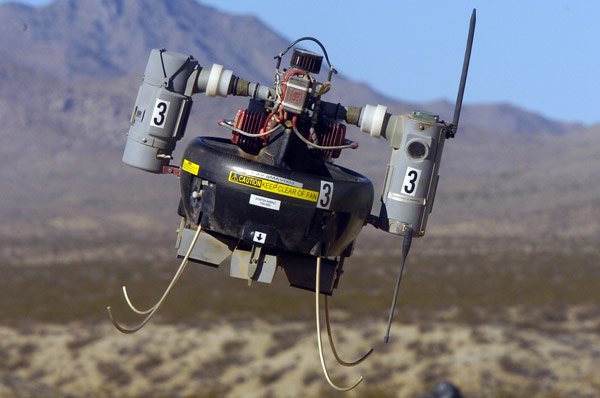
\includegraphics[scale=0.4]{images/fukushima.jpg}
	\caption{An example of UAV. T-Hawk, a US-made UAV, commonly used to search for roadside bombs in Iraq, made its debut when it photographed the Fukushima nuclear plant from above, providing a detailed look at the interior damage.}
	\label{fig:application}
\end{SCfigure}  

\noindent Many typse of UAVs have been developed over the last years, in particular the quadrotor type \cite{Aalborg}. The aim of this thesis is to contribute to the develop of the so called \textit{Prometheus project}, a fully autonomus vertical takeoff and landing vehicle, able to perform indoor enviroment exploration and mapping. To do this, we were inspired from the film Prometheus, where drones are able to map an indoor cave. Of course, due to technology and budget limitations, the vehicle will not have the same performance, but will have in theory the same capabilities. As previously said, this thesis is only a part of the project, that has been divided in three main parts:

\begin{itemize}
	\item mechanical design and building of the UAV \cite{Carlos};
	\item mathematical model, system identification and control;
	\item usage of the sensors, mapping and navigation algorithms.
\end{itemize}

\noindent This thesis will focus on the second point, but briefly introductions will give also in the other two points, in particular in the mechanical design, necessary for develop a mathematical model. 

\begin{SCfigure}[\sidecaptionrelwidth][h]
	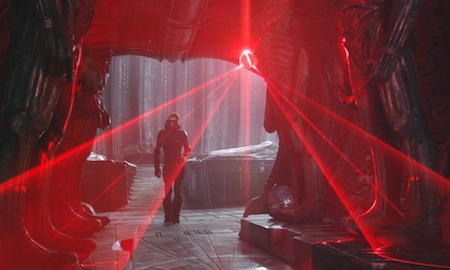
\includegraphics[scale=0.6]{images/prometheus_film.jpg}
	\caption{Frame of the prometheus movie, where the drone is performing the exploration and mapping of the cave.}
	\label{fig:prometheusFILM}
\end{SCfigure}

\noindent \textcolor{red}{Description of the varius chapters...}
	%%%%%%%%%%%%%%%%%%%%%%%%%%%%%%%%% INTRODUCTION %%%%%%%%%%%%%%%%%%%%%%%%%%%%%%%%%


	%%%%%%%%%%%%%%%%%%%%%%%%%%%%%%% DESIGN AND MODEL %%%%%%%%%%%%%%%%%%%%%%%%%%%%%%%
	\chapter{Design and model}
\label{designModel}

In this chapter we will focus in the description of the mechanical model of the UAV and the sensor system and, from these, a mathematical model will be derived, necessary for build and simulate a control law, and to perform system identification. In the end, we'll also describe the hardware and software used for the accomplish of this thesis.

\section{Mechanical design}
\label{mechanicalDesign}

The overall objective of the Prometheus project is navigation and mapping, for these we mean obtain a 3D reconstruction of an unknown indoor physical environment, using a 360 degrees \textit{Lidar} laser scanner, which, coupled to a quadrotor type UAV, will explore in a autonomous way. 

\begin{SCfigure}[\sidecaptionrelwidth][h]
	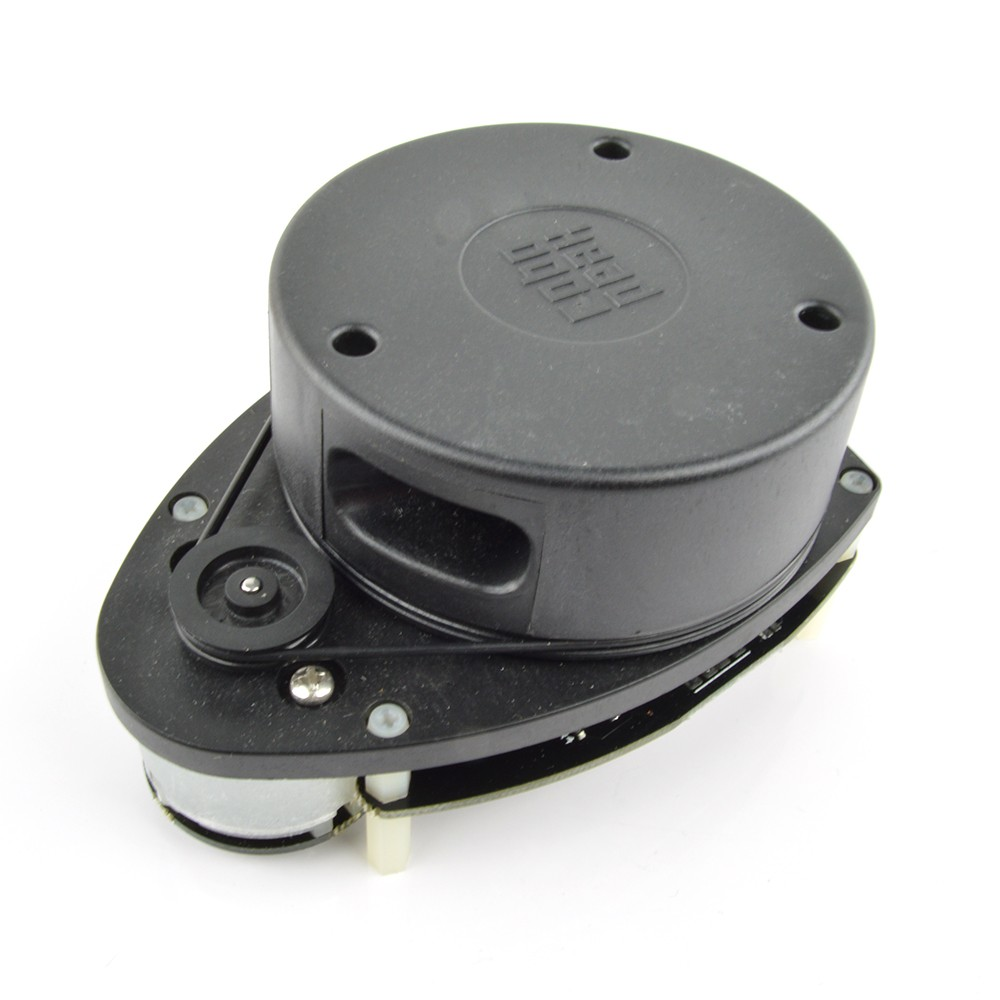
\includegraphics[scale=0.21]{images/lidar_laser.jpg}
	\caption{Lidar laser scanner, it is able to perform a 360 degrees mapping.}
	\label{fig:lidar}
\end{SCfigure}

\noindent Lidar is a surveying technology that measures distance by illuminating a target with a laser light. Lidar is an acronym of \textit{Light Detection And Ranging}, (sometimes \textit{Light Imaging, Detection, And Ranging}). Lidar is popularly used as a technology to make high-resolution maps, with applications in geodesy, geomatics, archeology, geography, geology, geomorphology, seismology, forestry, atmospheric physics and so on. What is known as Lidar is sometimes simply referred to as laser scanning or 3D scanning, with terrestrial, airborne and mobile applications\footnote{\url{https://en.wikipedia.org/wiki/Lidar}}. The specific Lidar laser scanner used in this project is depict in figure \ref{fig:lidar}, where is possible to see the rotating structure moved by a motor attached in the bottom of the frame. However, this sensor is only able to perform 2D mapping and, attached to a drone, make it practically impossible to perform a complete 3D mapping. To solve this problem, several approaches could be adopted, such as use a more complicated and more expensive sensor, that can maps directly in 3D, or just by simply use more than one Lidar. However, the solution adopted in this project is again inspired from the movie Prometheus, where the sensor is also rotating around the UAV. In such a way, the Lidar has three degrees of freedom in the movement and a 3D mapping can be performed. This solution comports, of course,the usage of only one laser scanner, but require a rotating structure that can move the sensor.

\begin{figure}[h]
	\centering
	\begin{subfigure}[t]{0.49\textwidth}
		\centering
		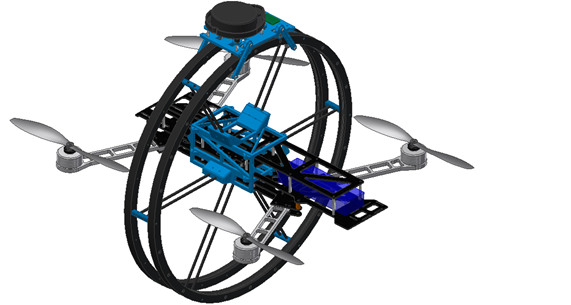
\includegraphics[scale = 0.45]{images/render1.png}
		\caption{Render of the entire vehicle.}
		\label{subfig:render1}
	\end{subfigure} 
	\begin{subfigure}[t]{0.49\textwidth}
		\centering
		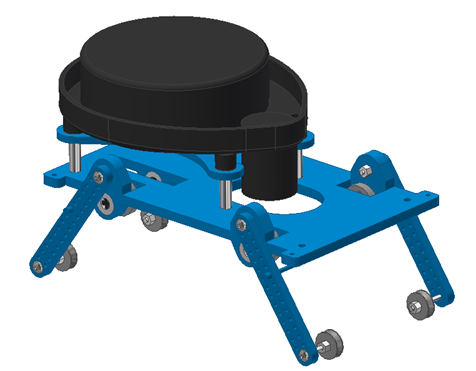
\includegraphics[scale = 0.5]{images/render2.png}
		\caption{Render of the moving cart.}
		\label{subfig:render2}
	\end{subfigure}
	\caption{Renders of the UAV and of the cart.}
	\label{fig:renders}
\end{figure}

\noindent In figure \ref{subfig:render1} is possible to see clearly the platform, made of two lightweight rings, and the cart that provides the circular movement of the sensor. An important choice was also the selection of the UAV, that has to guarantee to flight also with the weight of the mechanical structure, sensor and all the electronics needed to fly and control the movement of the cart.

\section{Mathematical model}
\label{mathematicalModel}

Is pretty much clear from the previous section that this UAV is different from almost every other vehicle that is possible to buy, this of course require a complete and detailed study to characterize the mathematical model. For characterize the model, is before necessary to provide some definitions, that are also valid for standard commercial quadrotors.

\begin{figure}[h]
	\centering
	\tdplotsetmaincoords{50}{-60} % 50 -60
		
	\def \semiaxis  {0.8}					% from center to propeller (diag)
	\def \centers {\semiaxis}		        % x and y of centers
	\def \body {\semiaxis / 5}				% half diagonal of body
	\def \height {0.05}						% half height of body
	\def \propeller {0.3}					% radius of propeller
	\def \innerpropeller {0.05}				% radius inner circle propeller
	\def \heightpropeller {0.05}			% height propeller plane
		
	\begin{tikzpicture}[scale=4,tdplot_main_coords]
		
		% axis
		\draw[line width=3pt] (-\centers, 0, 0) -- (\centers, 0, 0);	
		\draw[line width=3pt] (0, \centers, 0) -- (0, -\centers, 0);

		% propellers
		\tdplotdrawarc[thick, fill=gray] {(0, \centers, \heightpropeller)}{\propeller}{0}{360}{}{}
		\tdplotdrawarc[thick, fill=gray] {(\centers, 0, \heightpropeller)}{\propeller}{0}{360}{}{}
		\tdplotdrawarc[thick, fill=gray] {(0, -\centers, \heightpropeller)}{\propeller}{0}{360}{}{}
		\tdplotdrawarc[thick, fill=gray] {(-\centers, 0, \heightpropeller)}{\propeller}{0}{360}{}{}

		% center propellers
		\tdplotdrawarc[fill] {(0, \centers, \heightpropeller)}{\innerpropeller}{0}{360}{}{}
		\tdplotdrawarc[fill] {(\centers, 0, \heightpropeller)}{\innerpropeller}{0}{360}{}{}
		\tdplotdrawarc[fill] {(0, -\centers, \heightpropeller)}{\innerpropeller}{0}{360}{}{}
		\tdplotdrawarc[fill] {(-\centers, 0, \heightpropeller)}{\innerpropeller}{0}{360}{}{}

		% body
		\fill (\body,\body,\height) -- (\body,-\body,\height) -- (-\body,-\body,\height) -- (-\body,\body,\height) -- cycle;
		\fill (\body,\body,-\height) -- (\body,-\body,-\height) -- (-\body,-\body,-\height) -- (-\body,\body,-\height) -- cycle; % down
		\fill (-\body,-\body,-\height) -- (-\body,-\body,\height) -- (-\body,\body,\height) -- (-\body,\body,-\height) -- cycle; % back
		\fill (\body,\body,-\height) -- (\body,\body,\height) -- (\body,-\body,\height) -- (\body,-\body,-\height) -- cycle; % front
		\fill (\body,-\body,-\height) -- (\body,-\body,\height) -- (-\body,-\body,\height) -- (-\body,-\body,-\height) -- cycle; % left
		\fill (\body,\body,-\height) -- (\body,\body,\height) -- (-\body,\body,\height) -- (-\body,\body,-\height) -- cycle; % right
		
		% Coordinate frame
		\coordinate (O) at (0,0,0) node[red, anchor = north]{$O_B$};
		\draw[ultra thick,->,red] (0,0,0) -- (-1,-1,0) node[anchor=north west]{$x_B$};
		\draw[ultra thick,->,red] (0,0,0) -- (-1,1,0) node[anchor=south west]{$y_B$};
		\draw[ultra thick,->,red] (0,0,0) -- (0,0,1) node[anchor=south]{$z_B$};

		% Rotors arrows
		\draw [->, ultra thick] (\centers+0.2, 0, \heightpropeller) arc (0:300:0.2);
		\draw [->, ultra thick] (-\centers+0.2, 0, \heightpropeller) arc (0:300:0.2);
		\draw [<-, ultra thick] (0.2, \centers, \heightpropeller) arc (0:300:0.2);
		\draw [<-, ultra thick] (0.2, -\centers, \heightpropeller) arc (0:300:0.2);				
	\end{tikzpicture}
	\caption{Sketch of a standard quadrotor with its body frame attach.}
	\label{fig:quadrtotor}
\end{figure}

\noindent A quadrotor helicopter is made of a central frame and four propellers that are attach to the frame with respectively four arms. Moreover, the propellers' rotation direction must be opposite in pairs, like illustrated in figure \ref{fig:quadrtotor}. \newline
\noindent Furthermore, is necessary to define two frames, the \textit{world fixed frame} and the \textit{body frame} attached to the vehicle.
\noindent In figure \ref{fig:frames} is possible to see the two frames, the world frame, in black, is fixed to a point and it can't be moved, the body frame, in blue, instead is attached to the quadrotor and can move with six degrees of freedom, that are position and orientation. In this, we are interesting in knowing the translation and rotation of the body frame in respect to the world frame. For represent the translation, a three dimension vector $\mathbf{x}$ is enough, that actually indicate the position of the quadrotor in the space. Instead, for the rotation, we used \textit{quaternions} \cite{quaternion}, that will be introduced in the following section.

\begin{figure}[h]
	\centering
	\begin{tikzpicture}[]

		\def \length {2}
		\def \xbody {5}
		\def \ybody {0}

		% World frame
		\draw[rotate=30] (0, 0, 0) -- (0, 0, 0) node[anchor=north west]{$O_W$};
		\draw[->, ultra thick] (0, 0, 0) -- (\length, 0, 0) node[anchor=north west]{$x_W$};
		\draw[->, ultra thick] (0, 0, 0) -- (0, \length, 0) node[anchor=north west]{$z_W$};
		\draw[->, ultra thick] (0, 0, 0) -- (0, 0, \length) node[anchor=north west]{$y_W$};

		% Body frame
		\draw[rotate=30] (\xbody, \ybody, 0) -- (\xbody, \ybody, 0) node[anchor=north west, blue]{$O_B$};
		\draw[->, ultra thick, blue, rotate=30] (\xbody, \ybody, 0) -- (\xbody+\length, \ybody, 0) node[anchor=north west]{$x_B$};
		\draw[->, ultra thick, blue, rotate=30] (\xbody, \ybody, 0) -- (\xbody, \ybody+\length, 0) node[anchor=north east]{$z_B$};
		\draw[->, ultra thick, blue, rotate=30] (\xbody, \ybody, 0) -- (\xbody, \ybody, \length) node[anchor=north west]{$y_B$};

		\draw[-, dashed, rotate=30] (0, 0, 0) -- (\xbody, \ybody, 0);

	\end{tikzpicture}
	\caption{Illustration of the world and body frames.}
	\label{fig:frames}
\end{figure}
	
\subsection{Quaternion math}
\label{quaternion}

A quaternion is a hyper complex number of rank 4, which can be represented as follow

\begin{equation}
	\mathbf{q} = 
	\begin{bmatrix}
		q_0 & q_1 & q_2 & q_3
	\end{bmatrix}^T
	\label{eq:quatDef}
\end{equation}

\noindent The quaternion units from $q_1$ to $q_3$ are called the vector part of the quaternion, while $q_0$ is the scalar part \cite{EmilQuaternion}. Multiplication of two quaternions $\mathbf{p}$ and $\mathbf{q}$, is being performed by the \textit{Kronecker product}, denoted as $\otimes$. If $\mathbf{p}$ represents one rotation and $\mathbf{q}$ represents another rotation, then $\mathbf{p} \otimes \mathbf{q}$ represents the combined rotation.

\begin{align}
	\mathbf{p} \otimes \mathbf{q} &=
	\begin{bmatrix}
		p_0q_0 - p_1q_1 - p_2q_2 - p_3q_3 \\
		p_0q_1 + p_1q_0 + p_2q_3 - p_3q_2 \\
		p_0q_2 - p_1q_3 + p_2q_0 + p_3q_1 \\
		p_0q_3 + p_1q_2 - p_2q_1 + p_3q_0
	\end{bmatrix} \\
	&= Q(\mathbf{p})\mathbf{q} =
	\begin{bmatrix}
		p_0 & -p_1 & -p_2 & -p_3 \\
		p_1 & p_0  & -p_3 & p_2 \\
		p_2 & p_3  & p_0  & -p_1 \\
		p_3 & -p2  & p_1  & p_0
	\end{bmatrix}
	\begin{bmatrix}
		q_0 \\
		q_1 \\
		q_2 \\
		q_3
	\end{bmatrix} \\
	&= \bar{Q}(\mathbf{q})\mathbf{p} = 
	\begin{bmatrix}
		q_0 & -q_1 & -q_2 & -q_3 \\
		q_1 & q_0  & q_3  & -q_2 \\
		q_2 & -q_3 & q_0  & q_1 \\
		q_3 & q_2  & -q_1 & q_0  
	\end{bmatrix}
	\begin{bmatrix}
		p_0 \\
		p_1 \\
		p_2 \\
		p_3
	\end{bmatrix}
	\label{eq:quatKronecker}
\end{align}

\noindent The norm of a quaternion is defined as

\begin{equation}
	||\mathbf{q}|| = \sqrt{q_0^2 + q_1^2 + q_2^2 + q_3^2} 
	\label{eq:quatNorm}
\end{equation}

\noindent If the norm of the quaternion is equal to $1$, then the quaternion is called \textit{unit quaternion}. The complex conjugate of a quaternion has the same definition as normal complex numbers.

\begin{equation}
	\mathbf{q}^* = 
	\begin{bmatrix}
		q_0 & -q_1 & -q_2 & -q_3
	\end{bmatrix}^T
	\label{eq:quatConj}
\end{equation}

\noindent The inverse of a quaternion is defined as a normal inverse of a complex number.

\begin{equation}
	\mathbf{q}^{-1} = \frac{\mathbf{q}^*}{||\mathbf{q}||^2}
	\label{eq:quatInverse}
\end{equation}

\noindent The time derivative of the unit quaternion is the vector of \textit{quaternion rates} \cite{quaternion2}. It requires some algebraic manipulation but is important to notice that the quaternion rates, $\dot{\mathbf{q}}$, are related to the angular velocity $\boldsymbol{\omega} = \begin{bmatrix} \omega_x & \omega_y & \omega_z \end{bmatrix}^T$. It can be represented in two ways:

\begin{itemize}
		
	\item as in equation \eqref{eq:quatDerivative1} in case that the angular velocity is in the world frame (subscript $W$)
	\begin{equation}
		\dot{\mathbf{q}}_{\boldsymbol{\omega}_W}(\mathbf{q}, \boldsymbol{\omega}_W) = \frac{1}{2}\mathbf{q}\otimes
		\begin{bmatrix}
			0 \\
			\boldsymbol{\omega}_W
		\end{bmatrix}
		= \frac{1}{2}Q(\mathbf{q})
		\begin{bmatrix}
			0 \\
			\boldsymbol{\omega}_W
		\end{bmatrix}
		\label{eq:quatDerivative1}
	\end{equation}

	\item as in equation \eqref{eq:quatDerivative2} if the angular velocity vector is in the body frame of reference (subscript $B$).

	\begin{equation}
		\dot{\mathbf{q}}_{\boldsymbol{\omega}_B}(\mathbf{q}, \boldsymbol{\omega}_B) = \frac{1}{2}
		\begin{bmatrix}
			0 \\
			\boldsymbol{\omega}_B
		\end{bmatrix}
		\otimes \mathbf{q} = \frac{1}{2}\bar{Q}(\mathbf{q})
		\begin{bmatrix}
			0 \\
			\boldsymbol{\omega}_B
		\end{bmatrix}
		\label{eq:quatDerivative2}
	\end{equation}
\end{itemize}

\noindent A unit quaternion can be used also as a rotation operator, however the transformation requires both the quaternion and its conjugate, as show in equation \eqref{eq:quatRotateVector}. This rotates the vector $\mathbf{v}$ from the world frame to the body frame represented by $\mathbf{q}$.

\begin{equation}
	\boldsymbol{\omega} = \mathbf{q} \otimes 
	\begin{bmatrix}
		0 \\
		\mathbf{v}
	\end{bmatrix}
	\otimes \mathbf{q}^*
	\label{eq:quatRotateVector}
\end{equation}

\noindent Unit quaternion can be use also to represents \textit{rotation matrices}. Consider a vector $\mathbf{v}_W$ in the world frame. If $\mathbf{v}_B$ is the same vector in the body coordinates, then the following relations hold

\begin{align}
	\begin{bmatrix}
		0 \\
		\mathbf{v}_B
	\end{bmatrix}
	&= \mathbf{q} \cdot
	\begin{bmatrix}
		0 \\
		\mathbf{v}_W
	\end{bmatrix}
	\cdot \mathbf{q}^* \\
	&= \bar{Q}(\mathbf{q})^T Q(\mathbf{q})
	\begin{bmatrix}
		0 \\
		\mathbf{v}_W
	\end{bmatrix} \\
	&=
	\begin{bmatrix}
		1          & \mathbf{0}^T \\
		\mathbf{0} & R_{\mathbf{q}}(\mathbf{q})
	\end{bmatrix}
	\begin{bmatrix}
		0 \\
		\mathbf{v}_W
	\end{bmatrix}
	\label{eq:quatRotationMatrix1}
\end{align}

\noindent where

\begin{equation}
	R_{\mathbf{q}}(\mathbf{q}) =
	\begin{bmatrix}
		q_0^2+q_1^2-q_2^2-q_3^2 & 2q_1q_2+2q_0q_3         & 2q_1q_3-2q_0q_2 \\
		2q_1q_2-2q_0q_3         & q_0^2-q_1^2+q_2^2-q_3^2 & 2q_2q_3+2q_0q_1 \\
		2q_1q_3+2q_0q_2         & 2q_2q_3-2q_0q_1         & q_0^2-q_1^2-q_2^2+q_3^2
	\end{bmatrix}
	\label{eq:quatRotationMatrix2}
\end{equation}

\noindent That is,

\begin{align}
	\mathbf{v}_B &= R_{\mathbf{q}}(\mathbf{q})\mathbf{v}_W \\
	\mathbf{v}_W &= R_{\mathbf{q}}(\mathbf{q})^T\mathbf{v}_B
	\label{eq:quatRotationMatrix3}
\end{align}

\noindent Just as with rotation matrices, sequences of rotations are represented by products of quaternions. That is, for unit quaternions $\mathbf{q}$ and $\mathbf{p}$, it holds that

\begin{equation}
	R_{\mathbf{q}}(\mathbf{q} \cdot \mathbf{p}) = R_{\mathbf{q}}(\mathbf{q})R_{\mathbf{q}}(\mathbf{p})
	\label{eq:quatRotationMatrix4}
\end{equation}

\noindent Finally, for representing quaternion rotations in a more intuitive manner, the conversion from Euler angles (roll $\phi$, pitch $\theta$ and yaw $\psi$) to quaternion and vice versa can be performed by utilizing the following two equations respectively.

\begin{gather}
	q = 
	\begin{bmatrix}
		\cos{(\phi/2)}\cos{(\theta/2)}\cos{(\psi/2)} + \sin{(\phi/2)}\sin{(\theta/2)}\sin{(\psi/2)} \\
		\sin{(\phi/2)}\cos{(\theta/2)}\cos{(\psi/2)} - \cos{(\phi/2)}\sin{(\theta/2)}\sin{(\psi/2)} \\
		\cos{(\phi/2)}\sin{(\theta/2)}\cos{(\psi/2)} + \sin{(\phi/2)}\cos{(\theta/2)}\sin{(\psi/2)} \\
		\cos{(\phi/2)}\cos{(\theta/2)}\sin{(\psi/2)} - \sin{(\phi/2)}\sin{(\theta/2)}\cos{(\psi/2)} 
	\end{bmatrix} \\
	\begin{bmatrix}
		\phi \\
		\theta \\
		\psi
	\end{bmatrix}
	=
	\begin{bmatrix}
		\atan2(2(q_0q_1+q_2q_3), q_0^2-q_1^2-q_2^2+q_3^2) \\
		\asin(2(q_0q_2-q_3q_1)) \\
		\atan2(2(q_0q_3+q_1q_2), q_0^2+q_1^2-q_2^2-q_3^2)
	\end{bmatrix}
	\label{eq:quatEuler}
\end{gather}

\phantom{x} % necessary to place the next figure

\subsection{Quadrotor modeling}
\label{quadModel}

We consider first a standard quadrotor, without a rotating platform, like in figure \ref{fig:quadrtotorVectors}. 

\begin{figure}[!h]
	\centering
	\tdplotsetmaincoords{60}{-135} % 60 -135
		
	\def \semiaxis  {0.8}			    	% from center to propeller (diag)
	\def \centers {\semiaxis}		        % x and y of centers
	\def \body {\semiaxis / 5}				% half diagonal of body
	\def \height {0.05}						% half height of body
	\def \propeller {0.3}					% radius of propeller
	\def \innerpropeller {0.05}				% radius inner circle propeller
	\def \heightpropeller {0.05}			% height propeller plane
		
	\begin{tikzpicture}[scale=4,tdplot_main_coords]
		
		% axis
		\draw[line width=3pt] (-\centers, 0, 0) -- (\centers, 0, 0);	
		\draw[line width=3pt] (0, \centers, 0) -- (0, -\centers, 0);

		% propellers
		\tdplotdrawarc[thick, fill=gray] {(0, \centers, \heightpropeller)}{\propeller}{0}{360}{}{}
		\tdplotdrawarc[thick, fill=gray] {(\centers, 0, \heightpropeller)}{\propeller}{0}{360}{}{}
		\tdplotdrawarc[thick, fill=gray] {(0, -\centers, \heightpropeller)}{\propeller}{0}{360}{}{}
		\tdplotdrawarc[thick, fill=gray] {(-\centers, 0, \heightpropeller)}{\propeller}{0}{360}{}{}

		% center propellers
		\tdplotdrawarc[fill] {(0, \centers, \heightpropeller)}{\innerpropeller}{0}{360}{}{}
		\tdplotdrawarc[fill] {(\centers, 0, \heightpropeller)}{\innerpropeller}{0}{360}{}{}
		\tdplotdrawarc[fill] {(0, -\centers, \heightpropeller)}{\innerpropeller}{0}{360}{}{}
		\tdplotdrawarc[fill] {(-\centers, 0, \heightpropeller)}{\innerpropeller}{0}{360}{}{}

		% body
		\fill (\body,\body,\height) -- (\body,-\body,\height) -- (-\body,-\body,\height) -- (-\body,\body,\height) -- cycle;
		\fill (\body,\body,-\height) -- (\body,-\body,-\height) -- (-\body,-\body,-\height) -- (-\body,\body,-\height) -- cycle; % down
		\fill (-\body,-\body,-\height) -- (-\body,-\body,\height) -- (-\body,\body,\height) -- (-\body,\body,-\height) -- cycle; % back
		\fill (\body,\body,-\height) -- (\body,\body,\height) -- (\body,-\body,\height) -- (\body,-\body,-\height) -- cycle; % front
		\fill (\body,-\body,-\height) -- (\body,-\body,\height) -- (-\body,-\body,\height) -- (-\body,-\body,-\height) -- cycle; % left
		\fill (\body,\body,-\height) -- (\body,\body,\height) -- (-\body,\body,\height) -- (-\body,\body,-\height) -- cycle; % right
		
		% Coordinate frame
		\coordinate (O) at (0,0,0) node[red, anchor=east]{$O_B$};
		\draw[ultra thick,->,red] (0,0,0) -- (0,-1.6,0) node[anchor=south west]{$x_B$};
		\draw[ultra thick,->,red] (0,0,0) -- (1.6,0,0) node[anchor=east]{$y_B$};
		\draw[ultra thick,->,red] (0,0,0) -- (0,0,1.4) node[anchor=south]{$z_B$};

		% Rotors arrows
		\draw [->, ultra thick] (\centers+0.2, 0, \heightpropeller) arc (0:300:0.2) node[anchor=south west]{$\Omega_4$};
		\draw [->, ultra thick] (-\centers+0.2, 0, \heightpropeller) arc (0:300:0.2) node[anchor=south west]{$\Omega_2$};
		\draw [<-, ultra thick] (0.2, \centers, \heightpropeller) arc (0:300:0.2) node[anchor=south west]{$\Omega_3$};
		\draw [<-, ultra thick] (0.2, -\centers, \heightpropeller) arc (0:300:0.2) node[anchor=south west]{$\Omega_1$};

		% Force arrows
		\draw[ultra thick,->,blue] (0, \centers, \heightpropeller) -- (0, \centers, \heightpropeller+0.4) node[anchor=east]{$f_3$};
		\draw[ultra thick,->,blue] (\centers, 0, \heightpropeller) -- (\centers, 0, \heightpropeller+0.4) node[anchor=east]{$f_4$};
		\draw[ultra thick,->,blue] (0, -\centers, \heightpropeller) -- (0, -\centers, \heightpropeller+0.4) node[anchor=east]{$f_1$};
		\draw[ultra thick,->,blue] (-\centers, 0, \heightpropeller) -- (-\centers, 0, \heightpropeller+0.4) node[anchor=east]{$f_2$};

		% Torque arrows
        \draw[->, ultra thick, canvas is zy plane at x=\centers+0.6, orange] (0.15, 0, 0) arc (0:360:0.15) node[anchor=south east]{$\tau_y$};
        \draw[->, ultra thick, canvas is zx plane at y=-\centers-0.6, orange] (0.15, 0, 0) arc (0:360:0.15) node[anchor=south east]{$\tau_x$};
        \draw[->, ultra thick, orange] (0.15, 0, 0.6) arc (0:360:0.15) node[anchor=south east]{$\tau_z$};

	\end{tikzpicture}
	\caption{Sketch of a standard quadrotor.}
	\label{fig:quadrtotorVectors}
\end{figure}

\noindent In figure \ref{fig:quadrtotorVectors} are also impressed the force vectors $F_i$ generate from each motor-propeller, the torques vectors $\tau_x$, $\tau_y$ and $\tau_z$ about the three axis and the propeller's speed $\Omega_i$. Now, for modeling the rigid body of a multirotor, the standard \textit{Newton-Euler kinematics} equations can be utilized \cite{Bresciani}.

\begin{equation}
	\begin{bmatrix}
		\mathbf{f} \\
		\boldsymbol{\tau}
	\end{bmatrix}
	=
	\begin{bmatrix}
		m \cdot I_{3\times 3} & \mathbf{0} \\
		\mathbf{0}^T & I_{cm}
	\end{bmatrix}
	\begin{bmatrix}
		\mathbf{\ddot{x}_B} \\
		\boldsymbol{\dot{\omega}_B}
	\end{bmatrix}
	+
	\begin{bmatrix}
		\mathbf{0} \\
		\boldsymbol{\omega_B} \times I_{cm} \cdot \boldsymbol{\omega_B}
	\end{bmatrix}
	\label{eq:NewtonEuler}
\end{equation}

\noindent Where $\mathbf{f} = \begin{bmatrix} f_x & f_y & f_z \end{bmatrix}^T$ is the vector of the total force, $\boldsymbol{\tau} = \begin{bmatrix} \tau_x & \tau_y & \tau_z \end{bmatrix}^T$ is the total torque, $m$ is the mass of the quadrotor, $I_{cm}$ is the matrix of inertia related to the center of mass, $\mathbf{\ddot{x}_B}$ is the acceleration of the quadrotor center of mass related to the body frame and $\boldsymbol{\omega_B} = \begin{bmatrix} \omega_x & \omega_y & \omega_z \end{bmatrix}^T$ is the rotational rates in the body frame.

\noindent Before deriving the torque relationship, the motors' models from the input signal to the thrust force are needed. In specific, the four input signals are the speed of the propellers $u_i$, map between $0$ (no throttle) and $1$ (full throttle). Then, the thrust for each propeller can be simply derive as follow

\begin{equation}
	f_i(t) = a_{f,i} \Omega_i^2 = a_{f,i}\Omega_{max, i}^2 u_i(t)^2
	\label{eq:motorThrust}
\end{equation}

\noindent where $a_{f,i} \in \rm I\!R_+$ are the thrust constants of the motor-propeller combination, $\Omega_{max, i} \in \rm I\!R_+$ are the maximum rotational speed of the motors and $u_i(t)$ are the motors' signals. What is missing in equation \eqref{eq:motorThrust} is the model of the DC motors and in particular, a map between the input signal $u_i(t)$ and the control signal $u_{in,i}(t)$. To keep the model simple but still accurate\footnote{\url{http://pi19404.github.io/pyVision/2015/04/10/25/}}, the motor has been modeled like a delay, like in equation \eqref{eq:motorDelay}.

\begin{equation}
	u_i(t) \approx \frac{1}{\tau_i s+1}u_{in.i}(t)
	\label{eq:motorDelay}
\end{equation}

\noindent This approach is very common \cite{motor}, since all the parameters of a motor are not provide from datasheet, especially from cheap motors that is possible to find quite often in a commercial quadrotor. Furthermore, to represent the direction of the thrust from a motor it should be considered that 

\begin{align}
	\mathbf{f}_i(t) &= a_{f,i} \Omega_{max,i}^2u_i(t)\mathbf{n}_i \label{eq:propellerDirection1} \\
	\mathbf{n}_i &= R_i \cdot 
	\begin{bmatrix} 
		0 & 0 & 1 
	\end{bmatrix}^T 
	\label{eq:propellerDirection2}
\end{align} 

\noindent Where, in this case, $\mathbf{f}_i(t)$ is the force vector for each propeller and $R_i$ is the rotational matrix encoding the direction of the thrust and torque vector. Then the torque representation is given by

\begin{equation}
	\boldsymbol{\tau}_i(t) = -\sgn(\Omega_i)b_{f,i}\Omega_{max,i}^2u_i(t)^2\mathbf{n}_i
	\label{eq:motorTorque}
\end{equation}

\noindent where $b_{f,i} \in \rm I\!R_+$ is the torque constant.

\noindent Now, by defining the vector $\mathbf{l}_i = \begin{bmatrix} l_{x,i} & l_{y,i} & l_{z,i} \end{bmatrix}^T$ the distance between the \textit{center of mass} and the position where the propeller $i$ is attached, combining equations \eqref{eq:propellerDirection1}, \eqref{eq:propellerDirection2} and \eqref{eq:motorTorque} is possible to obtain equation \eqref{eq:forceTorque} as in the work \cite{modelIdentification}.

\begin{equation}
	\begin{bmatrix}
		\mathbf{f}_{total} \\
		\boldsymbol{\tau}_{total}
	\end{bmatrix}
	=
	\begin{bmatrix}
		\sum\limits_{i=1}^{4} \mathbf{f}_i(u_i^2) \\
		\sum\limits_{i=1}^{4} \mathbf{l}_i \times \mathbf{f}_i(u_i^2) + \boldsymbol{\tau}_i(u_i^2)
	\end{bmatrix}
	\label{eq:forceTorque}
\end{equation}

\noindent This combined with the Newton-Euler kinematics of equation \eqref{eq:NewtonEuler} gives the final model, from control signal to acceleration and angular acceleration, as depicted in equations \eqref{eq:finalModel1} and \eqref{eq:finalModel2}.

\begin{equation}
	\begin{split}
		\begin{bmatrix}
			\ddot{\mathbf{x}}_B \\
			\dot{\boldsymbol{\omega}}_B
		\end{bmatrix}
		&=
		\begin{bmatrix}
			\dots & \frac{a_{f,i}\Omega_{max,i}^2\mathbf{n}_i}{m} & \dots \\
			\dots & I_{cm}^{-1}\Big[ (\mathbf{l}_i+\boldsymbol{\Delta l})\times a_{f,i}\Omega^2_{max,i}\mathbf{n}_i-\sgn(\Omega_i)b_{f,i}\Omega_{max,i}^2\mathbf{n}_i\Big] & \dots
		\end{bmatrix}
		\begin{bmatrix}
			\vdots \\
			u_i^2 \\
			\vdots
		\end{bmatrix}
		+ \\
		&+
		\begin{bmatrix}
			\mathbf{0} \\
			I_{cm}^{-1}\bigl(\boldsymbol{\omega}_B \times I_{cm} \boldsymbol{\omega}_B \bigl)
		\end{bmatrix} \\
	\end{split}
	\label{eq:finalModel1}
\end{equation}

\begin{equation}
	u_i = \frac{1}{\tau_is+1}u_{in,1}
	\label{eq:finalModel2}
\end{equation}

\noindent Where $\boldsymbol{\Delta l}$ is the offset vector of the \textit{center of gravity} (\textit{CoG}) in the body frame of reference. From the model \eqref{eq:finalModel1} the linear and angular accelerations are given, is then necessary to convert those from the body frame and integrate to obtain the position $\mathbf{x}_W$ and orientation $\mathbf{q}_W$ of the quadrotor with the respect to the world frame. Then, by adding the gravity term we have

\begin{equation}
	\ddot{\mathbf{x}}_{B, g} = R_{\mathbf{q}_W}(\mathbf{q}_W)^T \cdot
	\begin{bmatrix}
		0 \\
		0 \\
		-g 
	\end{bmatrix}
	+ \ddot{\mathbf{x}}_B
	\label{eq:gravity}
\end{equation}

\noindent  where $g$ is the gravity constant, about $9.81$, and $R_{\mathbf{q}_W}(\mathbf{q}_W)$ is the rotation matrix built from equation \eqref{eq:quatRotationMatrix2}. To derive the velocity $\dot{\mathbf{x}}_W$ in the world frame, once again by using the rotation matrix we obtain

\begin{equation}
	\dot{\mathbf{x}}_W = R_{\mathbf{q}_W}(\mathbf{q}_W)\cdot\dot{\mathbf{x}}_{B, g}
	\label{eq:velocityWorld}
\end{equation}

\noindent Instead, for the orientation, we use the results from the paragraph \ref{quaternion} and we get

\begin{equation}
	\dot{\mathbf{q}}_W = \frac{1}{2}\cdot Q(\boldsymbol{\omega})\cdot\mathbf{q}_W
	\label{eq:orientation}
\end{equation}

\begin{figure}[h]
	\centering
	\begin{tikzpicture}[thick,scale=0.85, every node/.style={scale=0.85}]
		\coordinate (origin)  at (0,    0);
		\coordinate (input)   at (0,    3.02);
		\coordinate (motors)  at (1,    3);
		\coordinate (dynamic) at (4,    1.5);
		\coordinate (gravity) at (7,    3);
		\coordinate (integr1) at (7.3,  1.5);
		\coordinate (integr2) at (9.6,  3.7);
		\coordinate (bodywor) at (11.6, 1.5);
		\coordinate (integr3) at (14.6, 3.7);
		\coordinate (integr4) at (14.6, 1.5);		
		\coordinate (output1) at (16.6, 4.11);
		\coordinate (output2) at (16.6, 1.91);
		\coordinate (outfit1) at (16.1, 1.9);
		\coordinate (outfit2) at (6.3,  0.8);
		\coordinate (outfit3) at (8.8,  1.9);
		\coordinate (outfit4) at (3.3,  1);

		\node[draw, minimum width=2cm, minimum height=1.5cm, anchor=south west, align=center] (MOT) at (motors) {Motors\\\eqref{eq:finalModel2}};
		\node[draw, minimum width=2cm, minimum height=3cm, anchor=south west, align=center] (DYN) at (dynamic) {Quadrotor\\dynamic\\\eqref{eq:finalModel1}};
		\node[draw, minimum width=1.6cm, minimum height=1.5cm, anchor=south west, align=center] (GRA) at (gravity) {Gravity\\\eqref{eq:gravity}};
		\node[draw, minimum width=1cm, minimum height=0.8cm, anchor=south west, align=center, fill=red] (IN1) at (integr1) {$\frac{1}{s}$};
		\node[draw, minimum width=2cm, minimum height=3cm, anchor=south west, align=center] (BTW) at (bodywor) {Body\\to\\world\\\eqref{eq:velocityWorld}\eqref{eq:orientation}};
		\node[draw, minimum width=1cm, minimum height=0.8cm, anchor=south west, align=center, fill=red] (IN2) at (integr2) {$\frac{1}{s}$};
		\node[draw, minimum width=1cm, minimum height=0.8cm, anchor=south west, align=center, fill=red] (IN3) at (integr3) {$\frac{1}{s}$};
		\node[draw, minimum width=1cm, minimum height=0.8cm, anchor=south west, align=center, fill=red] (IN4) at (integr4) {$\frac{1}{s}$};

		\draw[->] ($(input) + (0, 0.75)$) -- node[above]{$\mathbf{u}_{in}$} ($(MOT.180)$);
		\draw[->] ($(MOT.0)$) -- node[above]{$\mathbf{u}$} ($(DYN.180) + (0, 0.75)$);
		\draw[->] ($(IN2.0)$) -- node[above]{$\dot{\mathbf{x}}_B$} ($(BTW.180) + (0, 1.1)$);
		\draw[->] ($(BTW.0) + (0, 1.1)$) -- node[above]{$\dot{\mathbf{x}}_W$} ($(IN3.180)$);
		\draw[->] ($(BTW.0) - (0, 1.1)$) -- node[above]{$\dot{\mathbf{q}}_W$} ($(IN4.180)$);
		\draw[->] ($(DYN.0) + (0, 1.1)$) -- node[above]{$\ddot{\mathbf{x}}_B$} ($(GRA.180) + (0, 0.35)$);
		\draw[->] ($(DYN.0) - (0, 1.1)$) -- node[above]{$\dot{\boldsymbol{\omega}}_B$} ($(IN1.180)$);
		\draw[->] ($(IN1.0)$) -- node[above]{$\boldsymbol{\omega}_B$} ($(BTW.180) - (0, 1.1)$);
		\draw[->] ($(GRA.0)$) - ++(0.5, 0) -- ++(0.5, 0) |- node[above]{$\ddot{\mathbf{x}}_{B, g}$}($(IN2.180)$); 
		\draw[->] ($(IN3.0)$) -- node[above]{$\mathbf{x}_W$} (output1);
		\draw[->] ($(IN4.0)$) -- node[above]{$\mathbf{q}_W$} (output2);
		\draw[-] (outfit1) |- (outfit2);
		\draw[->] (outfit2) |- ($(GRA.180) - (0, 0.35)$);
		\draw[-] (outfit3) |- (outfit4);
		\draw[->] (outfit4) |- ($(DYN.180) - (0, 0.75)$);

	\end{tikzpicture}
	\caption{Block diagram of the quadrotor dynamic.}
	\label{fig:quadDynBlock}
\end{figure}

\noindent In figure \ref{fig:quadDynBlock} is depicted a block diagram of the quadrotor dynamic, from the inputs $\mathbf{u}_{in}$, to position $\mathbf{x}_W$ and orientation $\mathbf{q}_W$ in the world frame.

\subsection{Adding the rotating platform}
\label{addPlatform}

Till now, all the model was designed for a standard quadrotor vehicle, what we want to do in this section is to add the model of the rotating platform, necessary for deduce a controller and simulate it.

\noindent The movement of the platform, introduces a time variant center of gravity, that is simply modeled with time variant vectors $\mathbf{l}_i(t)$, that identify the displacement of the center of the propeller $i$ with the respect of the CoG. If we know precisely the position of the CoG of the quadrotor (without the moving cart) and the position of the CoG of the cart, the result position can be computed.


\begin{figure}[h]
	\centering
	\begin{subfigure}[b]{0.45\textwidth}
		\centering
		\tdplotsetmaincoords{0}{45} % 70 280
		\tdplotsetrotatedcoords{0}{0}{-45}
		
		\def \semiaxis  {0.8}					% from center to propeller (diag)
		\def \centers {\semiaxis}		        % x and y of centers
		\def \body {\semiaxis / 5}				% half diagonal of body
		\def \height {0.05}						% half height of body
		\def \propeller {0.3}					% radius of propeller
		\def \innerpropeller {0.05}				% radius inner circle propeller
		\def \heightpropeller {0.05}			% height propeller plane
		\def \ring {0.8}                        % ring radious	

		\begin{tikzpicture}[scale=4,tdplot_main_coords]
			
			% axis
			\draw[line width=2pt] (-\centers, 0, 0) -- (\centers, 0, 0);	
			\draw[line width=2pt] (0, \centers, 0) -- (0, -\centers, 0);

			% propellers
			\tdplotdrawarc[thick, fill=gray, opacity=0.4] {(0, \centers, 0)}{\propeller}{0}{360}{}{}
			\tdplotdrawarc[thick, fill=gray, opacity=0.4] {(\centers, 0, 0)}{\propeller}{0}{360}{}{}
			\tdplotdrawarc[thick, fill=gray, opacity=0.4] {(0, -\centers, 0)}{\propeller}{0}{360}{}{}
			\tdplotdrawarc[thick, fill=gray, opacity=0.4] {(-\centers, 0, 0)}{\propeller}{0}{360}{}{}

			% center propellers
			\tdplotdrawarc[fill] {(0, \centers, 0)}{\innerpropeller}{0}{360}{}{}
			\tdplotdrawarc[fill] {(\centers, 0, 0)}{\innerpropeller}{0}{360}{}{}
			\tdplotdrawarc[fill] {(0, -\centers, 0)}{\innerpropeller}{0}{360}{}{}
			\tdplotdrawarc[fill] {(-\centers, 0, 0)}{\innerpropeller}{0}{360}{}{}

			% body
			\fill[opacity=0.2] (\body,\body,\height) -- (\body,-\body,\height) -- (-\body,-\body,\height) -- (-\body,\body,\height) -- cycle;
			\fill[opacity=0.2] (\body,\body,-\height) -- (\body,-\body,-\height) -- (-\body,-\body,-\height) -- (-\body,\body,-\height) -- cycle; % down
			\fill[opacity=0.2] (-\body,-\body,-\height) -- (-\body,-\body,\height) -- (-\body,\body,\height) -- (-\body,\body,-\height) -- cycle; % back
			\fill[opacity=0.2] (\body,\body,-\height) -- (\body,\body,\height) -- (\body,-\body,\height) -- (\body,-\body,-\height) -- cycle; % front
			\fill[opacity=0.2] (\body,-\body,-\height) -- (\body,-\body,\height) -- (-\body,-\body,\height) -- (-\body,-\body,-\height) -- cycle; % left
			\fill[opacity=0.2] (\body,\body,-\height) -- (\body,\body,\height) -- (-\body,\body,\height) -- (-\body,\body,-\height) -- cycle; % right

			% ring
			\draw[tdplot_rotated_coords, -, line width=3pt, canvas is zy plane at x=0, blue] (\ring, 0, 0) arc (0:360:\ring);

			% cart
			\shade[tdplot_rotated_coords, ball color=black] (0, \ring*0.866, \ring*0.5) circle (.08);

			% dashed lines
			\draw[dashed] (0, \centers, 0) -- node[below]{$\mathbf{l}_1$} (0.112, 0.112, 0.112);
			\draw[dashed] (\centers, 0, 0) -- node[above]{$\mathbf{l}_2$} (0.112, 0.112, 0.112);
			\draw[dashed] (-\centers, 0, 0) -- node[above]{$\mathbf{l}_4$} (0.112, 0.112, 0.112);
			\draw[dashed] (0, -\centers, 0) -- node[below]{$\mathbf{l}_3$} (0.112, 0.112, 0.112);

			\shade[tdplot_rotated_coords, ball color=orange] (0, 0.2*0.866, 0.2*0.5) circle (.04cm) node[anchor=south west]{\thinspace \thinspace \thinspace CoG};

			\shade[ball color=red] (0, 0, 0) circle (0.04cm);
		
		\end{tikzpicture}
		\label{fig:quadrtotorRingTop}
		\caption{Top view.}
	\end{subfigure}
	\qquad
	\begin{subfigure}[b]{0.45\textwidth}
		\centering	
		\tdplotsetmaincoords{90}{45} % 70 280
		\tdplotsetrotatedcoords{0}{0}{-45}
		
		\def \semiaxis  {0.8}					% from center to propeller (diag)
		\def \centers {\semiaxis}		        % x and y of centers
		\def \body {\semiaxis / 5}				% half diagonal of body
		\def \height {0.05}						% half height of body
		\def \propeller {0.3}					% radius of propeller
		\def \innerpropeller {0.05}				% radius inner circle propeller
		\def \heightpropeller {0.05}			% height propeller plane
		\def \ring {0.8}                        % ring radious	

		\begin{tikzpicture}[scale=4,tdplot_main_coords]
			
			% axis
			\draw[line width=2pt] (-\centers, 0, 0) -- (\centers, 0, 0);	
			\draw[line width=2pt] (0, \centers, 0) -- (0, -\centers, 0);

			% propellers
			\tdplotdrawarc[thick, fill=gray, opacity=0.4] {(0, \centers, 0)}{\propeller}{0}{360}{}{}
			\tdplotdrawarc[thick, fill=gray, opacity=0.4] {(\centers, 0, 0)}{\propeller}{0}{360}{}{}
			\tdplotdrawarc[thick, fill=gray, opacity=0.4] {(0, -\centers, 0)}{\propeller}{0}{360}{}{}
			\tdplotdrawarc[thick, fill=gray, opacity=0.4] {(-\centers, 0, 0)}{\propeller}{0}{360}{}{}

			% center propellers
			\tdplotdrawarc[fill] {(0, \centers, 0)}{\innerpropeller}{0}{360}{}{}
			\tdplotdrawarc[fill] {(\centers, 0, 0)}{\innerpropeller}{0}{360}{}{}
			\tdplotdrawarc[fill] {(0, -\centers, 0)}{\innerpropeller}{0}{360}{}{}
			\tdplotdrawarc[fill] {(-\centers, 0, 0)}{\innerpropeller}{0}{360}{}{}

			% body
			\fill[opacity=0.2] (\body,\body,\height) -- (\body,-\body,\height) -- (-\body,-\body,\height) -- (-\body,\body,\height) -- cycle;
			\fill[opacity=0.2] (\body,\body,-\height) -- (\body,-\body,-\height) -- (-\body,-\body,-\height) -- (-\body,\body,-\height) -- cycle; % down
			\fill[opacity=0.2] (-\body,-\body,-\height) -- (-\body,-\body,\height) -- (-\body,\body,\height) -- (-\body,\body,-\height) -- cycle; % back
			\fill[opacity=0.2] (\body,\body,-\height) -- (\body,\body,\height) -- (\body,-\body,\height) -- (\body,-\body,-\height) -- cycle; % front
			\fill[opacity=0.2] (\body,-\body,-\height) -- (\body,-\body,\height) -- (-\body,-\body,\height) -- (-\body,-\body,-\height) -- cycle; % left
			\fill[opacity=0.2] (\body,\body,-\height) -- (\body,\body,\height) -- (-\body,\body,\height) -- (-\body,\body,-\height) -- cycle; % right

			% ring
			\draw[tdplot_rotated_coords, -, line width=3pt, canvas is zy plane at x=0, blue] (\ring, 0, 0) arc (0:360:\ring);

			\draw[tdplot_rotated_coords, <-, line width=2pt, canvas is zy plane at x=0, rotate=60] (0.6, 0, 0) node[anchor=south]{$\gamma$} arc (0:30:0.6);

			% cart
			\shade[tdplot_rotated_coords, ball color=black] (0, \ring*0.866, \ring*0.5) circle (.08cm);

			% dashed lines
			\draw[tdplot_rotated_coords, dashed] (0, 0, 0) -- (0, \ring*0.866, \ring*0.5);
			\draw[dashed] (0, \centers, 0) -- (0.112, 0.112, 0.112);
			\draw[dashed] (\centers, 0, 0) -- (0.112, 0.112, 0.112);
			\draw[dashed] (-\centers, 0, 0) -- (0.112, 0.112, 0.112);
			\draw[dashed] (0, -\centers, 0) -- (0.112, 0.112, 0.112);

			\shade[tdplot_rotated_coords, ball color=orange] (0, 0.2*0.866, 0.2*0.5) circle (.04cm) node[anchor=south east]{CoG};

			\shade[ball color=red] (0, 0, 0) circle (0.04cm);

			\node [text=white] at (0, 0, -0.98) {};
		\end{tikzpicture}
		\caption{Side view.}
		\label{fig:quadrotorRingSide}
	\end{subfigure}
	\caption{Quadrotor with the rotating platform in blue, in red the CoG of the quadrotor and in orange the resulting CoG.}
	\label{fig:quadrotorRing}
\end{figure}

\noindent In figure \ref{fig:quadrotorRing} is illustrated how the resulting CoG change with the position of the cart, is possible to see also the four $\mathbf{l}_i(t)$ vectors in black dashed line. Then the position of the CoG is

\begin{equation}
	\mathbf{p} = \frac{1}{m}\cdot \bigl(m_{quad}\mathbf{p}_{quad} + m_{cart}\mathbf{p}_{cart}\bigl)	
	\label{eq:CoG}
\end{equation}

\noindent where $m=m_{quad}+m_{cart}$ is the sum of the mass of the quadrotor plus the mass of the moving cart, i.e. the total mass, $\mathbf{p}_{quad}$ is the position of the center of gravity of the quadrotor without the cart with the respect to the origin of the body frame (in general the quadrotor frame is not symmetrical) and $\mathbf{p}_{cart}$ is the position of the CoG of the cart with the respect to the body frame. Then the vectors $\mathbf{l}_i$ are just the distance between the center of the propeller $i$ and $\mathbf{p}$.

\noindent Another difference in using the rotating platform is that the moment of inertia $I_{cm}$ is not constant, but depend from the position $\gamma$ of the cart, like in figure \ref{fig:quadrotorRingSide}. This problem can be solved by using the detailed \textit{CAD model} of the entire vehicle, provided in \cite{Carlos}. From this is possible to deduce the inertia for various position, and then create a simple piecewise model. 

\noindent The movement of the sensor introduces also a centrifugal force in the vehicle. In particular, if $\mathbf{p}_{cart}$ is the vector that encode the position of the cart with the respect of the body frame, the Newton's law of motion for the cart in vector form is 

\begin{equation}
	\mathbf{f}_{cart}=m_{cart}\mathbf{a}_{cart}=m_{cart}\frac{d^2\mathbf{p}_{cart}}{dt^2}
	\label{eq:NewtonForce}
\end{equation}

\noindent By twice applying the transformation above from the stationary to the rotating frame, the absolute acceleration of the cart can be written as \cite{physics}

\begin{align}
	\frac{d^2\mathbf{p}_{cart}}{dt^2} &= \frac{\partial}{\partial t}\Big(\frac{d\mathbf{p}_{cart}}{dt}\Big)+\boldsymbol{\omega}\times\Big(\frac{d\mathbf{p}_{cart}}{dt}\Big) \nonumber \\
	&= \frac{\partial}{\partial t}\Big(\frac{\partial\mathbf{p}_{cart}}{\partial t}+\boldsymbol{\omega}\times\mathbf{p}_{cart}\Big)+\boldsymbol{\omega}\times\Big(\frac{\partial\mathbf{p}_{cart}}{\partial t}+\boldsymbol{\omega}\times\mathbf{p}_{cart}\Big)
	\label{eq:centrifugalAcceleration}
\end{align}

\noindent where in this case $\boldsymbol{\omega}$ is the angular velocity of the cart with the respect to the body frame. Expanding expression \eqref{eq:centrifugalAcceleration}, noting that the chain rule applies to differentiation of cross products, that the cross product is distributive over addition, and coupling with equation \eqref{eq:NewtonForce}, we have

\begin{equation}
	\mathbf{f}_{cart}=m_{cart}\frac{\partial^2\mathbf{p}_{cart}}{\partial t^2}+\underbrace{m_{cart}\frac{d\boldsymbol{\omega}}{dt}\times\mathbf{p}_{cart}}_{\text{Euler force}}+\underbrace{2m_{cart}\boldsymbol{\omega}\times\frac{\partial\mathbf{p}_{cart}}{\partial t}}_{\text{Coriolis force}}+\underbrace{m_{cart}\boldsymbol{\omega}\times\bigl(\boldsymbol{\omega}\times\mathbf{p}_{cart}\bigl)}_{\text{centrifugal force}}
	\label{eq:cartAllForces}
\end{equation}

\noindent That describe the so called \textit{Euler, Coriolis and centrifugal force} of the moving platform. To add this to the main model, we just simply need to sum up the vector $\mathbf{f}_{cart}$, divide by $m_{cart}$ to the equation \eqref{eq:finalModel1}, in the first three rows of the matrix, that regard the acceleration of the body frame

\begin{equation}
	\begin{split}
		\begin{bmatrix}
			\ddot{\mathbf{x}}_B \\
			\dot{\boldsymbol{\omega}}_B
		\end{bmatrix}
		&=
		\begin{bmatrix}
			\dots & \frac{A_{F,i}\Omega_{max,i}^2\mathbf{n}_i}{m} & \dots \\
			\dots & I_{cm}^{-1}\Big[ (\mathbf{l}_i+\boldsymbol{\Delta l})\times A_{F,i}\Omega^2_{max,i}\mathbf{n}_i-\sgn(\Omega_i)B_{F,i}\Omega_{max,i}^2\mathbf{n}_i\Big] & \dots
		\end{bmatrix}
		\begin{bmatrix}
			\vdots \\
			u_i^2 \\
			\vdots
		\end{bmatrix}
		+ \\
		&+
		\begin{bmatrix}
			\mathbf{0} \\
			I_{cm}^{-1}\bigl(\boldsymbol{\omega}_B \times I_{cm} \boldsymbol{\omega}_B \bigl)
		\end{bmatrix} 
		+
		\frac{1}{m_{cart}}
		\begin{bmatrix}
		\mathbf{f}_{cart} \\
		\mathbf{0}
		\end{bmatrix}
	\end{split}
	\label{eq:finalModelCart}
\end{equation}


\section{Experimental setup}

In this section we are going to introduce all the hardware and the software use in this project. 

\noindent Starting from the hardware, we used a main board develop entirely at Lule\r{a} University of Technology (LTU), the \textit{KFly}\footnote{\url{https://gitlab.com/korken89/KFly}}. In figure \ref{fig:KFly} is reported a picture of the KFly board. It is a small ($36\times 36$ mm) but powerful enough board able to perform all the operations needed during the flight.

\begin{figure}[h] 
	\centering
   	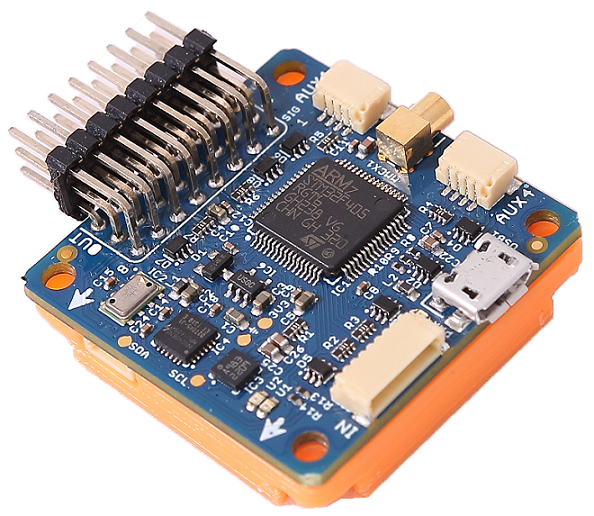
\includegraphics[scale = 0.45]{./images/KFly.png}
   	\caption{KFly board.}
   	\label{fig:KFly}
\end{figure} 

\noindent It is also equipped with different sensors, such an \textit{accelerometer} and a \textit{gyroscope} sensors, a \textit{magnetometer} and a \textit{pressure} sensors. With the accelerometer is possible to directly measured the acceleration in the body frame, while with the gyroscope is possible to directly measured the angular velocity. These two, combined with the magnetometer form a \textit{Inertial Measurement Unit} (\textit{IMU}). It is also equipped with 8 outputs (we will used 4 of them to control the motors) and 4 expansion connectors (3 UARTs and 1 CAN port) for the programming, communication, etcetera. For the communication between the vehicle and the base station, we used te \textit{XBee Pro} modules\footnote{\url{http://www.digi.com/lp/xbee}}.

\begin{figure}[h]
	\centering
	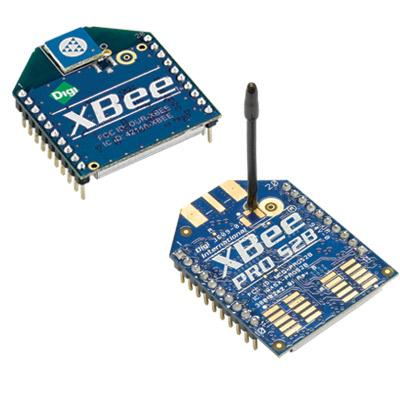
\includegraphics[scale = 0.6]{./images/XBee.jpg}
	\caption{XBee communication modules.}
	\label{fig:XBee}
\end{figure}

\noindent They have a built-in antenna, capable of a transmission range of theoretically 1000 meters. Moreover they have a maximum data rate of 250 kbps. Like previously said the UAV is equipped with a IMU, but to measure directly the pose of the vehicle we need other sensors. In particular, to test the control with extremely precision, we used a motion capture system. More precisely we used a \textit{Vicon}\footnote{\url{https://www.vicon.com/}} motion capture in the Field Robotics Lab (FROST) of LTU. The system is composed by 20 different cameras, mounted in the perimeter of the lab. By applying a number of markers in the object, is possible to track its position and orientation in the space, with a precision down to the tenth of millimeter.

\begin{figure}[h]
	\centering
	\begin{subfigure}[t]{0.49\textwidth}
		\centering
		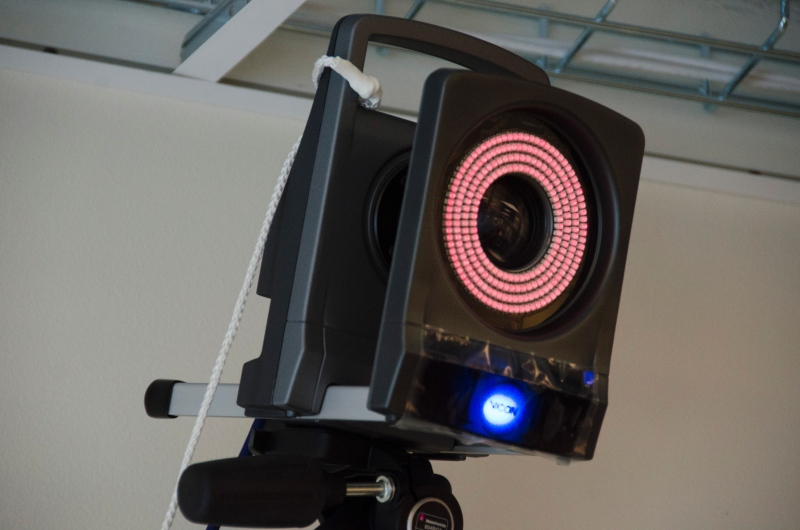
\includegraphics[scale = 0.25]{images/Vicon_camera.jpg}
		\caption{One Vicon camera.}
		\label{subfig:vicon1}
	\end{subfigure} 
	\begin{subfigure}[t]{0.49\textwidth}
		\centering
		\includegraphics[scale = 0.047]{images/Vicon_PC.jpg}
		\caption{Representation of objects in the Vicon system.}
		\label{subfig:vicon2}
	\end{subfigure}
	\caption{Vicon motion capture system.}
	\label{fig:vicon}
\end{figure} 

\begin{figure}[h]
	\centering
	\begin{subfigure}[t]{0.49\textwidth}
		\centering
		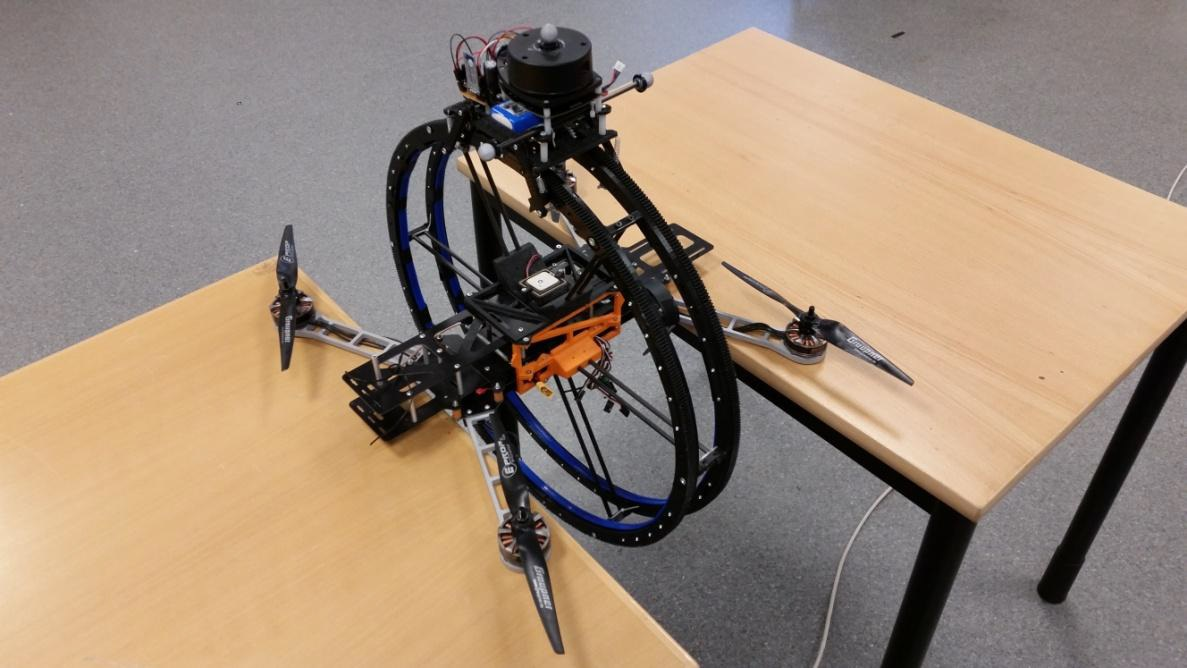
\includegraphics[scale = 0.22]{images/prometheus2.jpg}
		\label{subfig:prometheus1}
	\end{subfigure} 
	\begin{subfigure}[t]{0.49\textwidth}
		\centering
		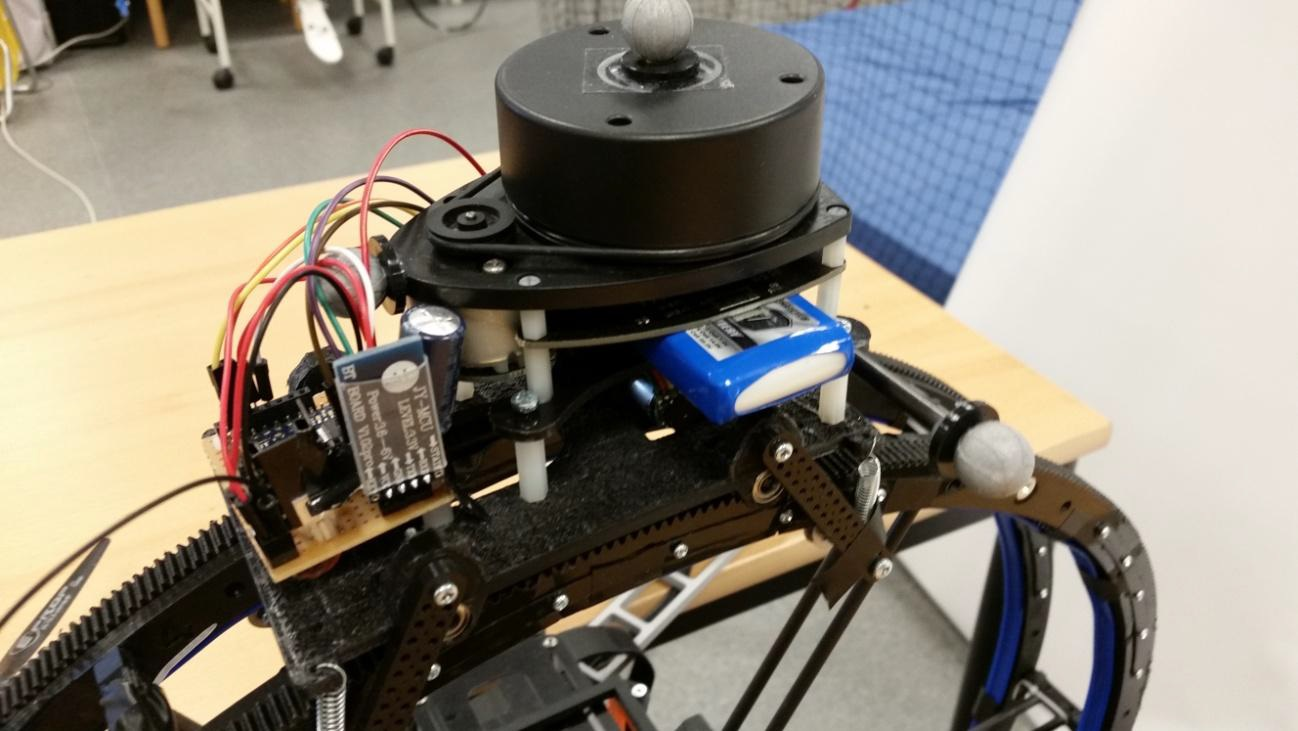
\includegraphics[scale = 0.2]{images/prometheus5.jpg}
		\label{subfig:prometheus2}
	\end{subfigure}
	\begin{subfigure}[t]{0.49\textwidth}
		\centering
		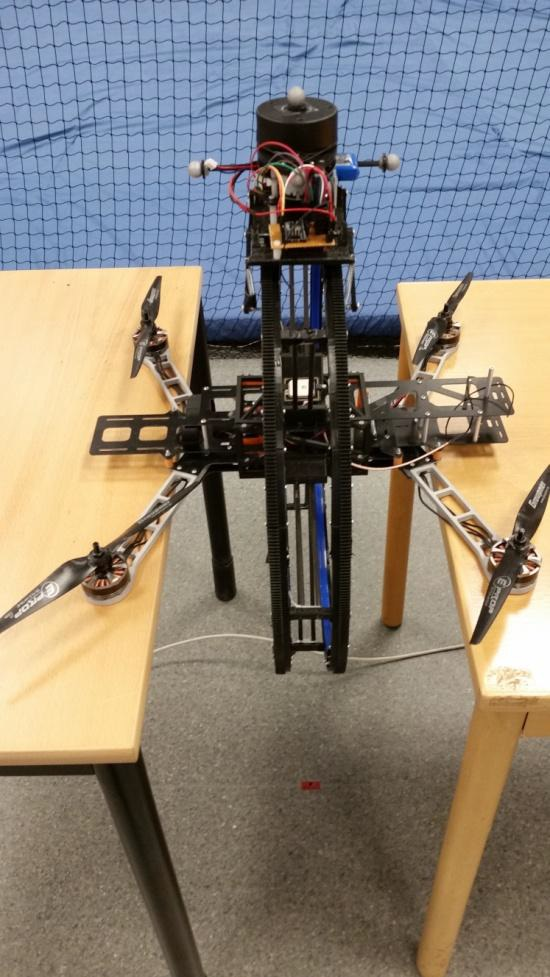
\includegraphics[scale = 0.3]{images/prometheus4.jpg}
		\label{subfig:prometheus3}
	\end{subfigure} 
	\begin{subfigure}[t]{0.49\textwidth}
		\centering
		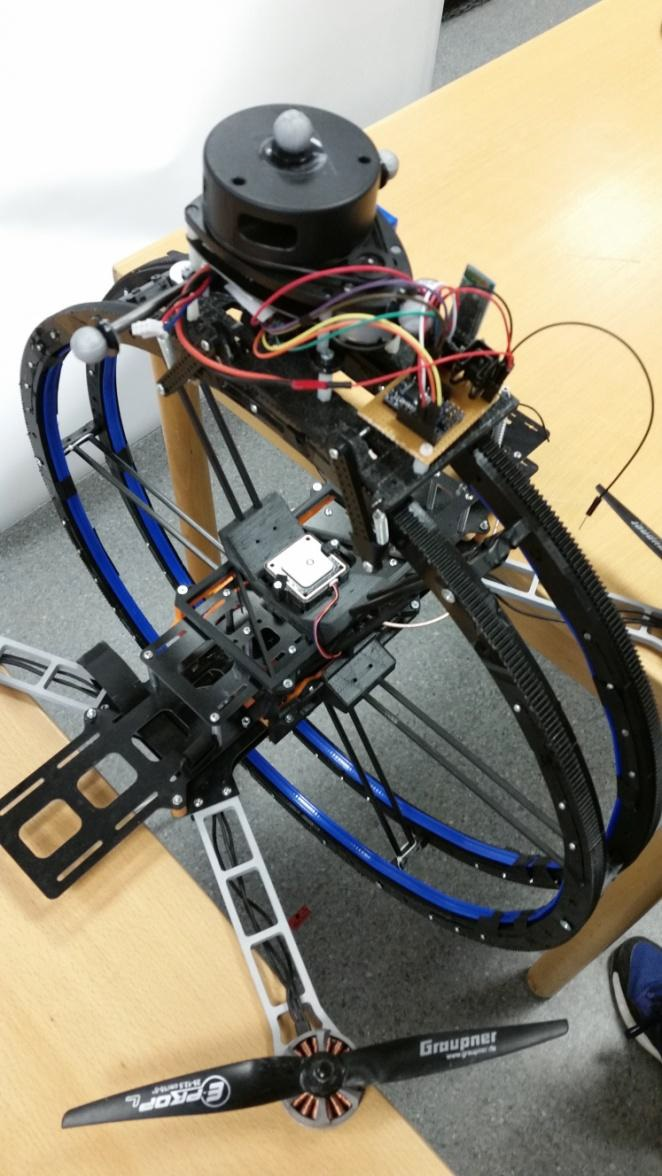
\includegraphics[scale = 0.25]{images/prometheus3.jpg}
		\label{subfig:prometheus4}
	\end{subfigure}
	\caption{First prototype of the Prometheus mapping drone.}
	\label{fig:prometheus}
\end{figure}

\noindent In figure \ref{fig:prometheus} there are some picture of the first prototype of the Prometheus mapping drone. In particular, is possible to see all the electronics and the Vicon markers on top and on the side of the Lidar sensor. These where useful during the test phase of the 3D mapping algorithm, in the third part of this project. Moving to the software part, all the simulations are made in a \textit{MATLAB} and \textit{SIMULINK} environment. This provided a fast and easy implementation of the control and system identification algorithms. Moreover, MATLAB is very useful for data analyzing after each flight. Instead, for the real application, we choose to use \textit{ROS}, the \textit{Robotic Operating System}\footnote{\url{http://www.ros.org/}} and then to rewrote all the code in \textit{C++}. ROS is an open source project that is a collection of software frameworks for robot software development, providing operating system-like functionality on a heterogeneous computer cluster. ROS provides standard operating system services such as hardware abstraction, low-level device control, implementation of commonly used functionality, message-passing between processes, and package management. It is very popular nowadays in robotic projects and there is a big worldwide community. However, due to its simplicity, the main problem was that the KFly couldn't run ROS onboard. We solve this problem by using a laptop with ROS install to run the control system, then send the control inputs to the KFly via XBee. By using this strategy we encounter problems with the bandwidth of the XBee, reaching its saturation limit, if we run the control algorithm at more than 50 Hertz, while the desire control rate was about 100 Hertz. A possible solution could be to use another low cost board, such as the \textit{Odroid c2}\footnote{\url{http://www.hardkernel.com/main/main.php}}, that can use high speed wi-fi link for the communication, and then practically unlimited bandwidth. Another important feature of the Odroid, is that it can run ROS onboard. This is extremely important in real world scenario, because run the control algorithm in remote could be very dangerous in case of signal lost, radio interference or other problems, and it can end up in a catastrophic failure of the entire system. In conclusion, ROS and the boards where powerful enough to run al the software in the loop, without any slowdown due to the workload of the control algorithm. This was achieved by using simple but efficacy solutions, as we will se in the next sections.   
	%%%%%%%%%%%%%%%%%%%%%%%%%%%%%%% DESIGN AND MODEL %%%%%%%%%%%%%%%%%%%%%%%%%%%%%%%



	%%%%%%%%%%%%%%%%%%%%%%%%%%%% SYSTEM IDENTIFICATION %%%%%%%%%%%%%%%%%%%%%%%%%%%%%
	\chapter{System identification}
\label{systemIdentification}

In this chapter, is about to be addressed an important part of this project. Since the model of the previous chapter is depending from many parameters, is necessary to identificate them, to be able to design an appropriate controller. A Kalman Filter approach will be used, based from the work \cite{modelIdentification}.

\section{System simplification and linear approximation}
\label{linearization}

Starting from the model deducted in section \ref{quadModel}

\begin{equation}
	\begin{split}
		\begin{bmatrix}
			\ddot{\mathbf{x}}_B \\
			\dot{\boldsymbol{\omega}}_B
		\end{bmatrix}
		&=
		\begin{bmatrix}
			\dots & \frac{a_{f,i}\Omega_{max,i}^2\mathbf{n}_i}{m} & \dots \\
			\dots & I_{cm}^{-1}\Big[ (\mathbf{l}_i+\boldsymbol{\Delta l})\times a_{f,i}\Omega^2_{max,i}\mathbf{n}_i-\sgn(\Omega_i)b_{f,i}\Omega_{max,i}^2\mathbf{n}_i\Big] & \dots
		\end{bmatrix}
		\begin{bmatrix}
			\vdots \\
			u_i^2 \\
			\vdots
		\end{bmatrix}
		+ \\
		&+
		\begin{bmatrix}
			\mathbf{0} \\
			I_{cm}^{-1}\bigl(\boldsymbol{\omega}_B \times I_{cm} \boldsymbol{\omega}_B \bigl)
		\end{bmatrix} \\
	\end{split}
	\label{eq:finalModel1a}
\end{equation}

\begin{equation}
	u_i = \frac{1}{\tau_is+1}u_{in,1}
	\label{eq:finalModel2a}
\end{equation}

\noindent we need to do some simplification. In particular, by assuming that all engines have the same parameters, is possible to rewrite these parameters as follows

\begin{align}
	a_{f,i}\Omega_{max,i}^2 &\approx a_f \\
	b_{f,i}\Omega_{max,i}^2 &\approx b_f \\
	\tau_i &\approx \tau
	\label{eq:simplification}
\end{align}

\noindent Moreover the term $I_{cm}^{-1}\bigl(\boldsymbol{\omega}\times I_{cm}\boldsymbol{\omega}_B\bigl)$ can be neglected \cite{modelIdentification}. This can be easily seen simply by simulating the mathematical model with and without the term, the differences are very small, as depicted in figure \ref{fig:comparisonOmega}. 

\begin{figure}[h]
	\centering
	\includestandalone[]{./chapter_3/plots/comparison}
	\caption{Simulation of the dynamic with and without the term $I_{cm}^{-1}\bigl(\boldsymbol{\omega}\times I_{cm}\boldsymbol{\omega}_B\bigl)$.}
	\label{fig:comparisonOmega}
\end{figure}

\noindent Another simplification, is that the inertia matrix $I_{cm}$ is a diagonal matrix, $I_{cm} = \diag(\allowbreak I_{xx}, I_{yy}, I_{zz})$. This is generally true in a standard quadrotor but is not so immediate for the vehicle of this project. However, if we align the $x$ axis with the orientation of the circular structure, we obtain a inertia matrix almost diagonal. What makes the matrix "less diagonal" is the position of the cart. However, the mass of the sensor is not sufficiently big to modify enough the matrix and this assumption is valid also here. Of course, in different applications, where the mass of the quadrotor and the mass of the sensor are more similar, a different approach is required. 

\noindent Another non linearity is in the inputs, since the model require the square of these. A solution of this problem proposed in \cite{modelIdentification} is to rewrite equation \eqref{eq:finalModel2a} with the square of the control inputs. This effectively moves the squared control signal from the force and torque equations to the input. This representation keeps the static relationship but will affect the dynamics of the first order system, but is assumed that a first order system still captures the majority of the dynamics. In conclusion, the approximate linear model is

\begin{gather}
	\begin{bmatrix}
		\ddot{\mathbf{x}}_B \\
		\dot{\boldsymbol{\omega}}_B
	\end{bmatrix}
	=
	\begin{bmatrix}
		\dots & \frac{a_f \mathbf{e}_3}{m} & \dots \\
		\dots & I_{cm}^{-1}\Big[(\mathbf{l}_i+\boldsymbol{\Delta l})\times a_f\mathbf{e}_3-\sgn(\Omega_i)b_f\mathbf{e}_3\Big] & \dots 
	\end{bmatrix}
	\begin{bmatrix}
		\vdots \\
		u_i \\
		\vdots
	\end{bmatrix} 
	\label{eq:linearModel1}\\
	u_i = \frac{1}{\tau s+1}u_{in,i}^2
	\label{eq:linearModel2}
\end{gather}

\noindent where instead of $\mathbf{n}_i$ there is $\mathbf{e}_3$ because in the structure of this particular vehicle, the propellers are mounted parallel to the ground and then with a force vector aligned to $\mathbf{e}_3=\begin{bmatrix}0 & 0 & 1\end{bmatrix}^T$.


\section{Quadrotor parameters}
\label{quadParameters}

From the simplified model of equations \eqref{eq:linearModel1} and \eqref{eq:linearModel2}, the identifiable parameters are 

\begin{equation}
	\boldsymbol{\beta} =
	\begin{bmatrix}
		\frac{a_f}{m} & \frac{a_f}{I_{xx}} & \frac{a_f}{I_{yy}} & \frac{b_f}{I_{zz}} & \Delta l_x & \Delta l_y 
	\end{bmatrix}^T, \hspace{10pt} \tau
	\label{eq:parameters}
\end{equation}

\noindent Then, is possible to rewrite the linear model in a more compact form:

\begin{equation}
	\begin{bmatrix}
		\ddot{\mathbf{x}}_B \\
		\dot{\boldsymbol{\omega}}_B
	\end{bmatrix}
	=
	\begin{bmatrix}
		L(\beta_1) \\
		A(\boldsymbol{\beta})
	\end{bmatrix}
	\mathbf{u}
	\label{eq:linearCompact}
\end{equation}

\noindent Under the assumption of the sampling rate to be much faster than the dynamics\footnote{In this case, thanks to the performance of the onboard electronics, the sampling rate is equal to $222$ Hertz.}, equation \eqref{eq:linearModel2} is implemented as discrete-time first order system, and the parameters are modeled as integrated white noise, which gives the following prediction equations

\begin{align}
	\boldsymbol{\omega}_{k} &= \boldsymbol{\omega}_{k-1}+\Delta t A(\boldsymbol{\beta}_{k-1})\mathbf{u}_{k-1} \\
    \mathbf{u}_k &= \frac{\tau_{k-1}}{\Delta t+\tau_{k-1}}\mathbf{u}_{k-1}+\frac{\Delta t}{\Delta t+\tau_{k-1}}\mathbf{u}_{in,k}^2 \\
    \boldsymbol{\beta}_k &= \boldsymbol{\beta}_{k-1} \\
    \tau_k &= \tau_{k-1}
\end{align}

\noindent where $\mathbf{u}_k$ and $\mathbf{u}_{in,k}$ are the inputs at time instant $k$ expressed in a vectorial way, $\Delta t$ is the sampling period and $\bullet^2$ is the element-wise square of a vector.


\section{Kalman filter}
\label{KalmanFilter}

A Kalman filter approach is chose for this project since it has good result in this kind of applications. Of course, better performances can be obtained with specific strategies for non linear systems \cite{parameterIdentification}, but these methods are in general much more complicated and require much more computational effort, especially if is necessary to estimate the parameters online.  

\noindent Now, is possible to use the standard Kalman filter equations \cite{KalmanFilter} to develop an online identification algorithm as follow.

\noindent The augmented state $\mathbf{x}_{est}$ is

\begin{equation}
	\mathbf{x}_{est}=
	\begin{bmatrix}
		\boldsymbol{\omega}_B & \mathbf{u}_{in} & \boldsymbol{\beta} & \tau
	\end{bmatrix}^T
	\in \rm I\!R^{15}
	\label{eq:augmentedState}
\end{equation} 

\noindent The initial values of $\boldsymbol{\omega}_B$ and $\mathbf{u}_{in}$ are know, so the state is initialized with these. Moreover, due to the parameters $\boldsymbol{\beta}$ and $\tau$ having a constraint to being positive, they are implemented as $\exp(\boldsymbol{\beta})$ and $\exp(\tau)$ to force positive results from the estimation, while the $\boldsymbol{\Delta l}$ are constrained to be within the propellers (the length of the arms is set to be equal to one, since the correct length is not necessary for the identification) which is implemented using a zero centered logistic function

\begin{equation}
	\frac{2}{1-\exp(-\boldsymbol{\Delta l})} -1
	\label{eq:logisticFunction}
\end{equation}

\noindent With the augmented state is possible to write a new state space system in discrete time with matrix $A_{est}$\footnote{For notation, $\mathbf{0}_{a\times b}$ is equal to a zero matrix with $a$ rows and $b$ columns,$\mathbf{1}_{a\times b}$ is equal to a ones matrix with $a$ rows and $b$ columns,$I_a$ is the identity matrix of dimension $a\times a$, and the vector $\mathbf{x}_{est,a:b}$ are the entries from $a$ to $b$ of the augmented state (is implicit that is consider at time $k$)}

\begin{align*}
	A_{\boldsymbol{\omega}, \mathbf{u}_{in}} &= 
	\left[
	\begin{array}{c}
		2\Delta te^{\beta_2}(\Delta l_y-1)\cdot\mathbf{u}^T \\
		\hline
		-2\Delta te^{\beta_3}(\Delta l_x+1)\cdot\mathbf{u}^T \\
		\hline
		-\sgn(\Omega_i)2\Delta te^{\beta_4}\cdot\mathbf{u}^T
	\end{array}
	\right] 
	& &\in \rm I\!R^{3\times 4} \\
	A_{\boldsymbol{\omega}, \boldsymbol{\beta}_1} &= \mathbf{0}_{3\times 1} & &\in \rm I\!R^{3\times 1}\\
	A_{\boldsymbol{\omega}, \boldsymbol{\beta}_{2}} &=
	\begin{bmatrix}
		\Delta te^{\beta_2}\bigg(\Delta l_y\sum\limits_{i=1}^{4}u_i^2-u_1^2-u_2^2+u_3^2+u_4^2\bigg) & 0 & 0
	\end{bmatrix}^T 
	& &\in \rm I\!R^{3\times 1}\\
	A_{\boldsymbol{\omega}, \boldsymbol{\beta}_{3}} &=
	\begin{bmatrix}
		0 & -\Delta te^{\beta_3}\bigg(\Delta l_y\sum\limits_{i=1}^{4}u_i^2+u_1^2-u_2^2-u_3^2+u_4^2\bigg) & 0
	\end{bmatrix}^T 
	& &\in \rm I\!R^{3\times 1}\\
	A_{\boldsymbol{\omega}, \boldsymbol{\beta}_{4}} &=
	\begin{bmatrix}
		0 & 0 & -\Delta te^{\beta_4}\sum\limits_{i=1}^{4}\sgn(\Omega_i)u_i^2
	\end{bmatrix}^T 
	& &\in \rm I\!R^{3\times 1}\\
	A_{\boldsymbol{\omega}, \boldsymbol{\beta}_{5}} &=
	\begin{bmatrix}
		0 & 0 & \Delta t
	\end{bmatrix}^T 
	& &\in \rm I\!R^{3\times 1}\\
	A_{\boldsymbol{\omega}, \boldsymbol{\beta}_{6:7}} &=
	\begin{bmatrix}
		0 & \Delta te^{\beta_2}\sum\limits_{i=1}^{4}u_i^2 \\ 
		-\Delta te^{\beta_3}\sum\limits_{i=1}^{4}u_i^2	& 0 \\
		0 & 0 
	\end{bmatrix} 
	& &\in \rm I\!R^{3\times 2}\\
	A_{\boldsymbol{\omega}, \boldsymbol{\beta}} &=
	\left[
	\begin{array}{c|c|c|c|c|c}
		A_{\boldsymbol{\omega}, \boldsymbol{\beta}_1} & A_{\boldsymbol{\omega}, \boldsymbol{\beta}_2} & A_{\boldsymbol{\omega}, \boldsymbol{\beta}_3} & A_{\boldsymbol{\omega}, \boldsymbol{\beta}_4} & A_{\boldsymbol{\omega}, \boldsymbol{\beta}_5} & A_{\boldsymbol{\omega}, \boldsymbol{\beta}_{6:7}}
	\end{array}
	\right]
	& &\in \rm I\!R^{3\times 7}\\
	A_{\mathbf{u}_{in}} &= \Big(1-\frac{\Delta t}{\Delta t+e^{\tau}}\Big)\cdot I_4 & &\in \rm I\!R^{4\times 4} \\
	A_{est,k} &=
	\left[ 
	\begin{array}{c}
		\begin{array}{c|c|c|c}
			I_{3} & A_{\boldsymbol{\omega}, \mathbf{u}_{in}} & A_{\boldsymbol{\omega}, \boldsymbol{\beta}} & \mathbf{0}_{3\times 1}
		\end{array} \\
		\hline
		\begin{array}{c|c|c}
			\mathbf{0}_{4\times 3} & A_{\mathbf{u}_{in}} & \mathbf{0}_{4\times 8}
		\end{array} \\
		\hline
		\begin{array}{c|c} 
			\mathbf{0}_{8\times7} & I_8
		\end{array}
	\end{array}
	\right]
	& &\in \rm I\!R^{15\times 15}
\end{align*}

\noindent and then use the Kalman filter equations in a recursive way \cite{KalmanFilter}

\begin{align*}
	P_k &= A_{est,k}\cdot P_{k-1}\cdot A_{est,k}^T + Q & \hspace{37pt} &\in \rm I\!R^{15\times 15} \\
	H_k &=
	\left[
		\begin{array}{c|c}
			I_3 & \mathbf{0}_{3\times 12} \\
			\hline
			\mathbf{0}_{1\times 3} & \begin{array}{c|c|c|c} 2e^{\beta_1}\cdot\mathbf{u}^T & \mathbf{0}_{1\times 2} & e^{\beta_1}\sum\limits_{i=1}^{4}u_i^2 & \mathbf{0}_{1\times 5} \end{array}
		\end{array}
	\right] & &\in \rm I\!R^{4\times 15} \\
	S_k &= H_k\cdot P_k\cdot H_k^T + R & &\in \rm I\!R^{4\times 4} \\
	K_k &= P_k\cdot H_k^T\cdot S_k^{-1} & &\in \rm I\!R^{15\times 4} \\
	P_k &= \big(I_{15} - K_k\cdot H_k\big)\cdot P_{k-1} & &\in \rm I\!R^{15\times 15} \\
	\mathbf{x}_{est,k} &= \mathbf{x}_{est,k-1} + K_k\cdot\Big(\begin{bmatrix}\boldsymbol{\omega} \\ \ddot{x}_z \end{bmatrix} - \begin{bmatrix}\mathbf{x}_{est,1:3} \\ e^{\beta_1}\cdot\mathbf{1}_{1\times 4}\cdot\mathbf{x}_{est,4:7}^2 \end{bmatrix}\Big) & &\in \rm I\!R^{15\times 1}
\end{align*}

\noindent where $P_k$ is the state update covariance matrix based on model, $H_k$ maps the measurement to the states, $S_k$ is the update measurement covariance, $K_k$ is the update Kalman gain, $Q\in\rm I\!R^{15\times 15}$ is the fixed covariance matrix and $R\in\rm I\!R^{4\times 4}$ the fixed measurement covariance matrix. Both $Q$ and $R$ are diagonal matrices.


\section{Results}
\label{resultsKalman}

\begin{figure}[h]
	\centering
 	\includestandalone[]{./chapter_3/plots/omega}
 	\caption{Measured and estimated angular rate, $\boldsymbol{\omega}_B$ and $\hat{\boldsymbol{\omega}}_B$.}
 	\label{fig:omegaKalman}		
\end{figure}

\noindent The estimator needs to be setup with specific process and measurement covariance $Q$ and $R$, and the starting state covariance $P_0$. The values for $Q$ and $P_0$ where found simply with a trial and error procedure, while $R$ was taken from the noise densities of the measured signals. In particular we measured a steady state position of the quadrotor, record the acceleration in the z axis $\ddot{x}_{B,z}$ and the angular rate $\boldsymbol{\omega}_B$, then by analyzing these data, a noise variance was extracted. Moreover, since in the augmented state $\mathbf{x}_{est}$ is present also an estimation of the angular rate $\hat{\boldsymbol{\omega}}$, to evaluate the quality of the estimation was also compare it with the measured angular rate. In this case the initial values of the state $\mathbf{x}_{est}$ were chose to be considerably different from a real value, just to show the performance of the estimator.

\begin{figure}[h]
	\centering
	\includestandalone[]{./chapter_3/plots/param_group_left}
	\includestandalone[]{./chapter_3/plots/param_group_right}
	\includestandalone[]{./chapter_3/plots/param_group_bottom}
	\caption{Estimated parameters $\boldsymbol{\beta}$ and $\tau$.}
	\label{fig:betaTauKalman}
\end{figure}

\noindent As is possible to see in figure \ref{fig:omegaKalman}, the estimation of the angular rate yields good results from the beginning for all the three axis. In figure \ref{fig:betaTauKalman} are instead plotted the estimations of all parameters $\boldsymbol{\beta}$ and $\tau$. The identification was performed with the cart fixed in one position. Is possible to see that for almost all parameters there is convergence after about $15$ seconds, while for the parameter $\frac{b_f}{I_{zz}}$ is necessary more time. This can be explain by observing the angular rate, in particular note that $\omega_z$ is almost zero for about the first 10 seconds, due to the particular trajectory of the vehicle. Of course, is not possible to perform system identification without excitation of the system and thats why the parameters depending on $\omega_z$ require more time to converge.

\noindent In conclusion the algorithm has been shown to work quite well, and for this application is not then necessary to use more sophisticated techniques.

	%%%%%%%%%%%%%%%%%%%%%%%%%%%% SYSTEM IDENTIFICATION %%%%%%%%%%%%%%%%%%%%%%%%%%%%%



	%%%%%%%%%%%%%%%%%%%%%%%%%%% TRAJECTORIES GENERATOR %%%%%%%%%%%%%%%%%%%%%%%%%%%%%
	\chapter{Trajectories generator}
\label{trajectoriesGenerator}

An important aspect of this project is the path plannig, because the aim is to map and navigate in a enviroment without a priori information and in complete autonomous. The study of path planning alghoritms and the sensor fusion to obtain the pose of the vehicle is not part of this thesis, however is part of this thesis to generate a trajectory for the UAV based on the output of a path planning algorithm. In particular, usually exploration algorithms provide only setpoints, not full trajectories \cite{potentialField} \cite{visionBasedMAV}. Is then necessary to provide a tool to generate possible trajectorie with constraints in the enviroment and in the dynamic of the vehicle. In this project we implemented the solution proposed in the work \cite{minimumSnap} and \cite{polyTraj}, where the author, after providing model and control, generate a trajectory composed by picewise polynomial functions.


\section{Trajectoy definition}
\label{trajDefinition}

In this work, a \textit{setpoint} $\boldsymbol{\sigma}_d$is define as a position in the space, $\mathbf{x}_d$, along a yaw angle, $\psi_d$, since in the next section we will control four degrees of freedom of the UAV, the position in the space and the yaw angle. We consider the problem of navigate through $m$ setpoints at specific time. A trivial trajectory is one that interpolate the setpoints using straight lines. However, such trajectory is inefficient because it require the quadrotor to come to a stop st each setpoint. This method generates trjectories that smoothly transition throught the setpoints at given times. We write down a trajectory as piecewise polynomial functions of order $n$ over $m$ time intervals

\begin{equation}
	\sigma_d(t)=
	\begin{cases}
		\sum\limits_{i=0}^{n}\sigma_{d,i,1}t^i & t_0 \le t < t_1 \\
		\sum\limits_{i=0}^{n}\sigma_{d,i,2}t^i & t_1 \le t < t_2 \\
		\vdots \\
		\sum\limits_{i=0}^{n}\sigma_{d,i,m}t^i & t_{m-1} \le t < t_m \\
	\end{cases}
	\label{eq:defTraj}
\end{equation}

\noindent where $\sigma_{d,i,j}$ is the coefficient of orden $i$ of the trajectory piece $j$ and $t_k$ is the time that the vehicle has to reach setpoint $k$, $i \in \begin{bmatrix}0 & n\end{bmatrix}$, $j \in \begin{bmatrix}1 & m\end{bmatrix}$, $k \in \begin{bmatrix}1 & m\end{bmatrix}$. The interest is then to minimize a cost function wich can be written using these piecewise polynomial. 

\begin{alignat}{3}
	\min\qquad & \int_{t_0}^{t_m}\mu_{\mathbf{x}} \Bigg|\Bigg|\frac{d^{k_{\mathbf{x}}}\mathbf{x}_d}{dt^{k_{\mathbf{x}}}} \Bigg|\Bigg|^2 + \mu_{\psi}\Bigg(\frac{d^{k_{\psi}}\psi_d}{dt^{k_{\psi}}}\Bigg)^2dt \\
	\text{subject to}\qquad & \boldsymbol{\sigma}_d(t_i) = \boldsymbol{\sigma}_{d,i}, && i=0,\dots ,m \nonumber \\
	& \frac{d^px_d}{dt^p}\Big|_{t=t_j}=0, && j=0,m; & p=1,\dots ,k_r \nonumber \\
	& \frac{d^py_d}{dt^p}\Big|_{t=t_j}=0, && j=0,m; & p=1,\dots ,k_r \nonumber \\
	& \frac{d^pz_d}{dt^p}\Big|_{t=t_j}=0, && j=0,m; & p=1,\dots ,k_r \nonumber \\
	& \frac{d^p\psi_d}{dt^p}\Big|_{t=tj}=0, && j=0,m; & p=1,\dots ,k_{\psi} \nonumber
	\label{eq:minimizationCost}
\end{alignat}

\noindent where $\mu_{\mathbf{x}}$ and $\mu_{\psi}$ are constants that make the integrand nondimensional. Here $\boldsymbol{\sigma}_d = \begin{bmatrix} x_d & y_d & z_d & \psi_d\end{bmatrix}^T$ and $\boldsymbol{\sigma}_{d,i}=\begin{bmatrix}x_{d,i} & y_{d,i} & z_{d,i} & \psi_{d,i}\end{bmatrix}^T$. We also assume that $t_0=0$ without loss of generality. The first constraint indicates that the result trajectory has to pass through the desire setpoints, while the rest of the constraints impose that all the derivatives at the initial and final point have to be zero (one can also set them to a specific value if necessary). By using the same choice of \cite{minimumSnap2}, we decide to minimize the snap for the position ($k_{\mathbf{x}}=4$) and the second derivative of the yaw angle ($k_{\psi}=2$). Now we want to formulate the trajectory generation problem as an optimization of a functional but in a finite dimensional setting. This will keep the computational effort very small to guarantee a real time application. In order to to this, we first write the constants $\boldsymbol{\sigma}_{d,i,j} =\begin{bmatrix}x_{d,i,j} & y_{d,i,j} & z_{d,i,j} & \psi_{d,i,j}\end{bmatrix}^T$ as a $4\cdot n\cdot m\times 1$ vector $\mathbf{c}$ with decision variables $\{x_{d,i,j} , y_{d,i,j} , z_{d,i,j} , \psi_{d,i,j}, i \in \begin{bmatrix}0 & n\end{bmatrix}, j \in \begin{bmatrix}0 & m\end{bmatrix}\}$. The trajectory generation preoblem \eqref{eq:minimizationCost} can be written in the form of a quadratic program (QP):

\begin{alignat}{2}
	\min\qquad & \mathbf{c}^TH\mathbf{c} + f^T\mathbf{c} \\
	\text{subject to}\qquad & A\mathbf{c} \le \mathbf{b} \nonumber \\
	& A_{eq}\mathbf{c} = \mathbf{b}_{eq} \nonumber
	\label{eq:quadraticProgram}
\end{alignat}

\noindent where the objective function will incorporate the minimization of the functional while the contraint can be used to satisfy constraints in the trajectory and it derivatives. A specification of an initial condition, final condition, or intermediate condition on any derivative of the trajectory (e.g. $\frac{d^kx_d}{dt^k}$) can be written as a row of the constraint $A_{eq}\mathbf{c} = \mathbf{b}_{eq}$. If conditions do not need to be
specified exactly then they can be represented with the inequality constraint $A\mathbf{c}\le \mathbf{b}$. 

\noindent Moreover, to simplify the problem, can be notice that in the cost function of equation \eqref{eq:minimizationCost}, the four dimension are indipendent, this means that the problem can be split in four different problem for each dimension. In such a way, the construction of the qudratic problem vectors and matrices will be considerable more simple. Furthermore, is possible to assume that each setpoint starts from $t_0=0$ and end to $t_j=1$. This because if we define a new time varible such as

\begin{equation}
	\tau = \frac{t-t_{j-1}}{t_j-t_{j-1}}
	\label{eq:simplyTime}
\end{equation}

\noindent the new one dimension position at time $\tau$ become

\begin{equation}
	x(\tau) = x(\frac{t-t_{j-1}}{t_j-t_{j-1}})	
\end{equation}

\noindent and its derivatives

\begin{align*}
	\frac{d}{dt}x(t) &= \frac{d}{dt}x(\tau) \\
	&= \frac{d}{d\tau}\frac{d\tau}{dt}x(\tau) \\
	&= \frac{1}{t_j-t_{j-1}}\frac{d}{d\tau}x(\tau) \\
	&... \\
	\frac{d^k}{dt^k}x(t) &= \frac{1}{(t_j-t_{j-1})^k}\frac{d^k}{d\tau^k}x(\tau)
\end{align*}

\noindent We can thus solve for each piecec of any piece-wise trajectory from $\tau=0$ to $1$, then scale to any $t_0$ to $t_j$.


\section{Optimization of a trajectory between two setpoints}

To make the derivation simpler, is better to start the optimization problem with only two setpoints and in only one dimension. In particular, the cost function become 

\begin{alignat}{2}
	J &= \int_{t_0}^{t_1}\Bigg|\Bigg|\frac{d^kx(t)}{dt}\Bigg|\Bigg|^2dt = \mathbf{c}^TH_{(t_0,t_1)}\mathbf{c} \\
	\text{subject to}\qquad & A\mathbf{c} = \mathbf{b} \nonumber
	\label{eq:oneSetpoint}
\end{alignat}

\noindent We can instead look for the non-dimensionalized trajectory $x(\tau)=c_n\tau^n+c_{n-1}\tau^{n-1}+\dots+c_1\tau+c_0$ where $\tau=\frac{t-t_0}{t_1-t_0}$. Note that this makes $\tau$ range from $0$ to $1$. Let $\mathbf{c}=\begin{bmatrix}c_n & c_{n-1} & \dots & c_1 & c_0\end{bmatrix}^T$.We can wite the cost function $J$ in term of the non-dimensionalized trajectory $x(\tau)$:

\begin{align}
	J &= \int_{t_0}^{t_1}\Bigg|\Bigg|\frac{d^kx(t)}{dt}\Bigg|\Bigg|^2dt \\
	&= \int_0^1\Bigg|\Bigg|\frac{1}{(t_1-t_0)^k}\frac{d^kx(\tau)}{d\tau}\Bigg|\Bigg|^2d(\tau(t_1-t_0)+t_0) \nonumber \\
	&= \frac{t_1-t_0}{(t_1-t_0)^{2k}}\int_0^1\Bigg|\Bigg|\frac{d^kx(\tau)}{d\tau}\Bigg|\Bigg|^2d\tau \nonumber \\
	&= \frac{1}{(t_1-t_0)^{2k-1}}\mathbf{c}^TH_{(0,1)}\mathbf{c} \nonumber \\
	&= \mathbf{c}^T\Bigg(\frac{1}{(t_1-t_0)^{2k-1}}H_{(0,1)}\Bigg)\mathbf{c} \nonumber
\end{align}

\noindent Thus, we want to minimize the cost function

\begin{alignat}{2}
	J &= \mathbf{c}^T\Bigg(\frac{1}{(t_1-t_0)^{2k-1}}H_{(0,1)}\Bigg)\mathbf{c} \\
	\text{subject to}\qquad & A\mathbf{c} = \mathbf{b} \nonumber
\end{alignat}

\noindent To find $H_{(0,1)}$, when $\mathbf{c}'=\begin{bmatrix}c_0 & c_1 & \dots & c_{n-1} & c_n\end{bmatrix}^T$, we can find $H'_{(0,1)}$ with:

\begin{align}
	H'[i,j]_{(t_0,t_11)} &=
	\begin{cases}
		\prod\limits_{z=0}^{k-1}(i-z)(j-z)\frac{t_1^{i+j-2k+1}-t_0^{i+j-2k+1}}{i+j-2k+1} & i\ge k \wedge j\ge k \\
		0 & i<k \vee j<k
	\end{cases} \label{eq:Htranspose} \\
	& i=0,\dots,n,\qquad j=0,\dots,n \nonumber
\end{align}

\noindent However, $\mathbf{c}=\begin{bmatrix}c_n & c_{n-1} & \dots & c_1 & c_0\end{bmatrix}^T$. Reflecting $H'$ from equation \eqref{eq:Htranspose} horizontally and vertcally will give the desire $H$ for the form of $\mathbf{c}$ we desire. The function to minimize is then $\Bigg(\frac{1}{(t_1-t_0)^{2k}}H_{(0,1)}\Bigg)$.

\noindent To find $A$

\begin{align*}
	A\mathbf{c} &= \mathbf{b} \\
	\begin{bmatrix}
		A(t_0) \\
		A(t_1) 
	\end{bmatrix}
	\mathbf{c} &=
	\begin{bmatrix}
		x(t_0) \\
		\vdots \\
		x^{(k-1)}(t_0) \\
		x(t_1) \\
		\vdots \\
		x^{(k-1)}(t_1)
	\end{bmatrix}
\end{align*}

\noindent Note that $A\mathbf{c}$ only contains rows where constraints are specified, if a condition is unconstrained just omit a row. Assuming that every condition is constrained, the general form of $A$ is:

\begin{align}
	A[i,j](t) &= 
	\begin{cases}
		\prod\limits_{z=0}^{i-1}(n-z-j)t^{n-j-i} & n-j \ge i \\
		0 & n-j<i
	\end{cases} \label{eq:matrixA} \\
	& i=0,\dots,r-1, \qquad j=0,\dots,n \nonumber
\end{align}

\noindent where $A[i,j]$ represents the $(n-j)$th coefficient of the $i$th derivative. In the non-dimensionalized case, we have $\tau_0=0$ and $\tau_1=1$:

\begin{equation}
	\begin{bmatrix}
		A(\tau_0) \\
		A(\tau_1) 
	\end{bmatrix}
	\mathbf{c} =
	\begin{bmatrix}
		x(t_0) \\
		\vdots \\
		(t_1-t_0)^{k-1}x^{(k-1)}(t_0) \\
		x(t_1) \\
		\vdots \\
		(t_1-t_0)^{k-1}x^{(k-1)}(t_1)
	\end{bmatrix}
\end{equation}


\section{Optimization of a trajectory between $m+1$ setpoints}

In this section, by recalling what we study in the previous section, is possible to derive the equations to optimize a trajectory for an arbitrary number of setpoints. In particular, we seek the piece-wise trajectory:

\begin{equation}
	x(t)=
	\begin{cases}
		x_1(t), & t_0\le t<t_1 \\
		x_2(t), & t_1\le t<t_2 \\
		\vdots \\
		x_m(t), & t_{m-1}\le t<t_m 	
	\end{cases}
\end{equation}

\noindent and continue to minimize the cost function

\begin{alignat}{2}
	J &= \int_{t_0}^{t_m}\Bigg|\Bigg|\frac{d^kx(t)}{dt}\Bigg|\Bigg|^2dt = \mathbf{c}^TH_{(t_0,t_m)}\mathbf{c} \\
	\text{subject to}\qquad & A\mathbf{c} = \mathbf{b} \nonumber
\end{alignat}

\noindent and again look for the non-dimensionalized trajectory

\begin{align}
	x(\tau) &=
	\begin{cases}
		x_1(\tau) = c_{1,n}\tau^n+\dots+c_{1,0}, & t_0\le t<t_1,\quad \tau=\frac{t-t_0}{t_1-t_0} \\
		x_m(\tau) = c_{m,n}\tau^n+\dots+c_{m,0}, & t_{m-1}\le t<t_m,\quad \tau=\frac{t-t_{m-1}}{t_m-t_{m-1}}
	\end{cases} \\
	& 0\le\tau<1 \nonumber
\end{align}

\noindent Let $\mathbf{c}_z=\begin{bmatrix}c_{z,n} & c_{z,n-1} & \dots & c_{z,1} & c_{z,0}\end{bmatrix}^T$ and $\mathbf{c}=\begin{bmatrix}\mathbf{c}_1^T & \mathbf{c}_2^T & \dots & \mathbf{c}_m^T\end{bmatrix}^T$. Each piece of the trajectory is optimized individually between $\tau_0=0$ and $\tau_1=1$. We want to minimize:

\begin{alignat}{2}
	J &= \int_{t_0}^{t_m}\Bigg|\Bigg|\frac{d^kx(t)}{dt}\Bigg|\Bigg|^2dt \\
	&= \sum\limits_{z=1}^m\int_{t_z-1}^{t_z}\Bigg|\Bigg|\frac{d^kx_z(t)}{dt}\Bigg|\Bigg|^2dt \nonumber \\
	&= \sum\limits_{z=1}^m\int_0^1\frac{t_z-t_{z-1}}{(t_z-t_{z-1})^{2k}}\Bigg|\Bigg|\frac{d^kx_z(\tau)}{d\tau}\Bigg|\Bigg|^2d\tau \nonumber \\
	&= \sum\limits_{z=1}^m \mathbf{c}_z^T\frac{1}{(t_z-t_{z-1})^{2k-1}}H_{(0,1)}\mathbf{c}_z \nonumber \\
	&= \mathbf{c}^TH\mathbf{c} \nonumber \\
	\text{subject to} \qquad & A\mathbf{c}=\mathbf{b} \nonumber
\end{alignat}

\noindent To find $H$, we recall that for each $\mathbf{c}'_z=\begin{bmatrix}c_{z,0} & c_{z,1} & \dots & c_{z,n-1} & c_{z,n} \end{bmatrix}^T$, where $z=1,\dots,m$, $H'_{(0,1)}$ is given by equation \eqref{eq:Htranspose}. Since $\mathbf{c}_z=\begin{bmatrix}c_{z,n} & c_{z,n-1} & \dots & c_{z,1} & c_{z,0}\end{bmatrix}^T$, refletting $H'$ horizzontally and vertically will give the desire $H$ for the form of $\mathbf{c}_k$. Is then possible to create the block diagonal matrix 

\begin{equation}
	H = 
	\begin{bmatrix}
		\frac{1}{(t_1-t_0)^{2k-1}}H_{(0,1)} & \dots & 0 & 0 \\
		 & \dots & \dots & \vdots \\
		\dots & 0 & \frac{1}{(t_{m-1}-t_{m-2})^{2k-1}}H_{(0,1)} & 0 \\
		0 & \dots & 0 & \frac{1}{(t_m-t_{m-1})^{2k-1}}H_{(0,1)}
	\end{bmatrix}	
\end{equation}

\noindent To find $A$, first, we need to account for endpoint constraints, in the non-dimensionalized case:

\begin{align}
	A_{endpoint}\mathbf{c} &= \mathbf{b}_{endpoint} \\
	\begin{bmatrix}
		A(\tau_0) & 0         & \dots & 0         \\
		A(\tau_1) & 0         & \dots & 0         \\
		0         & A(\tau_0) & \dots & 0         \\
		0         & A(\tau_1) & \dots & 0         \\
		\vdots    & 0         & \dots & \vdots    \\
		0         & \dots     & 0     & A(\tau_0) \\
		0         & \dots     & 0     & A(\tau_1)            
	\end{bmatrix}
	\mathbf{c} &= 
	\begin{bmatrix}
		x_1(t_0) 								\\
		\vdots   								\\
		(t_1-t_0)^{k-1}x_1^{(k-1)}(t_0) 		\\
		x_1(t_1) 								\\
		\vdots   								\\
		(t_1-t_0)^{k-1}x_1^{(k-1)}(t_1) 		\\
		\vdots   								\\
		x_m(t_{m-1}) 							\\
		\vdots                                  \\
		(t_m-t_{m-1})^{k-1}x_m^{(k-1)}(t_{m-1}) \\
		x_m(t_m)                                \\
		(t_m-t_{m-1})^{k-1}x_m^{(k-1)}(t_m)
	\end{bmatrix} \nonumber
\end{align}

\noindent Like before, we just omit rows where a condition is unconstrained. Also, note that except for constraints at $t_0$ and $t_m$, every other constraint must be include twice. The equation for $A[i,j](t)$ is the same of \eqref{eq:matrixA}

\noindent We must also take into account for constraints that ensure that when the trajectory switches from one piece to another at the sepoints, position and all the derivative lower than $k$ remain continuous, for a smooth path. In other words, is require that

\begin{align}
	A_{cont}\mathbf{c} &= \mathbf{b}_{cont} \\
	\begin{bmatrix}
		x_1(t_1)-x_2(t_2) 							  \\
		\vdots            							  \\
		x_1^{(k-1)}(t_1)-x_2^{(k-1)}(t_1) 			  \\
		\vdots                                        \\
		x_{m-1}(t_{m-1})-x_m(t_{m-1})                 \\
		\vdots                                        \\
		x_{m-1}^{(K-1)}(t_{m-1})-x_m^{(K-1)}(t_{m-1})
	\end{bmatrix} 
	&= 0 \nonumber
\end{align}

\noindent Translating to the non-dimeensionalized casa, $\tau_0=0$, $\tau_1=1$, and

\begin{align}
	A_{cont}\mathbf{c} &= \mathbf{b}_{cont} \\
	\begin{bmatrix}
		x_1(\tau_1)-x_2(\tau_2) \\
		\vdots \\
		\frac{1}{(t_1-t_0)^{k-1}}x_1^{(k-1)}(\tau_1)-\frac{1}{(t_2-t_1)^{k-1}}x_2^{(k-1)}(\tau_1) \\
		\vdots \\
		x_{m-1}(\tau_1)-x_m(\tau_0) \\
		\vdots \\
		\frac{1}{(t_{m-2}-t_{m-1})^{k-1}}x_{m-1}^{(K-1)}(\tau_1)-\frac{1}{(t_m-t_{m-1})^{k-1}}x_m^{(K-1)}(\tau_0)
	\end{bmatrix}
	&= 0 \nonumber
\end{align}

\noindent and then

\begin{equation}
	\begin{bmatrix}
		A_{cont}(t_1) & 0             & \dots & 0 \\
		0             & A_{cont}(t_2) &	\dots & 0 \\
		\vdots        & 0             & \dots & 0 \\
		0             & \dots         & 0     & A_{cont}(t_{m-1})  
	\end{bmatrix}
	\mathbf{c}=0
\end{equation}

\noindent where

\begin{align}
	A_{cont}[i,j](t_z) &=
	\begin{cases}
		\frac{1}{(t_z-t_{z-1})^i}\prod\limits_{z=0}^{i-1}(n-z-j)\tau_1^{n-j-i}, & n-j\ge i\wedge j\le n \\
		0,                                                                       & n-j<i\wedge j\le n   \\
		-\frac{1}{(t_{z+1}-t_z)^i}\prod\limits_{z=0}^{i-1}(1-z-j)\tau_0^{1-j-i}, & 1-j\ge i\wedge j>n   \\
		0,                                                                       & 1-j<i\wedge j>n      
	\end{cases} \\
	& i=0,\dots,k-1,\quad j=0,\dots,2(n+1) \nonumber 
\end{align}

\noindent The final constraints $A\mathbf{c}=\mathbf{b}$ take then the final form

\begin{align} 
	A\mathbf{c} &= \mathbf{b} \\
	\begin{bmatrix}
		A_{endpoint} \\
		A_{cont}
	\end{bmatrix}
	\mathbf{c} &=
	\begin{bmatrix}
		b_{endpoint} \\
		0
	\end{bmatrix} \nonumber	
\end{align}

\begin{figure}[h]
	\centering
 	\includestandalone[valign=t]{./chapter_4/plots/poly_group_left}
 	\includestandalone[valign=t]{./chapter_4/plots/poly_group_right}
 	\caption{Generated trajectory with its derivatives.}
 	\label{fig:polyTrajectory}		
\end{figure}

\noindent In figure \ref{fig:polyTrajectory} is reported the firt dimension of a generate trajectory evolving over the time. In particular in blue are plot the trajectory and its first four derivative, till the snap. Instead in black are plot the setpoints for the trajectory and the initial and final condition for each derivative, that are equal to zero. Notice that between setpoints two and three, the trajectory is not as expected, in the sense that first tend to go far from the desire setpoint and than reach it. That's because this is only one dimension of a more complex three dimension trajectory.

\section{Adding corridor constraints}

In this section, corridors constraints will add in the cost function \eqref{eq:minimizationCost}. For corridor constraints, we mean that the desire trajectory must be inside a corridor, this why for a safe obstacle avoidance and navigation algorithm, the vehicle must respect distance between walls and obstacles. To do this, we first define $\mathbf{u}_i$ as the unit vector along the segment from setpoint $\mathbf{r}_i$ and setpoint $\mathbf{r}_{i+1}$. 

\begin{equation}
	\mathbf{u}_i=\frac{\mathbf{r}_{i+1}-\mathbf{r}}{||\mathbf{r}_{i+1}-\mathbf{r}||}
	\label{eq:unitVector}
\end{equation}

\noindent The perpendicular distance vector, $\mathbf{d}_i(t)$, from segment $i$ is define as

\begin{equation}
	\mathbf{d}_i(t) = (\mathbf{r}_d(t)-\mathbf{r}_i)-((\mathbf{r}_d(t)-\mathbf{r}_i)\cdot\mathbf{t}_i)\mathbf{u}_i		
	\label{eq:perpendicularVector}	
\end{equation}

\noindent where $\mathbf{r}_d(t)$ is the desire trajectory at istant $t$. A corridor width on the infinity norm, $\delta_{i}$, is define for each corridor as follow

\begin{equation}
	\big|\big|\mathbf{d}_i(t)\big|\big|_{\infty}\le\delta_i \quad \text{while} \quad t_i\le t\le t_{i+1}
	\label{eq:corridorWidth}
\end{equation}

\noindent The reason to write the constraint like that, is because it can be incorporate into the QP problem by introducing $n_c$ intermediate points as

\begin{equation}
	\Bigg|x_a\cdot\mathbf{d}_i\Big(t_i+\frac{j}{1+n_c}(t_{i+1}-t_i)\Big)\Bigg|\le\delta_i \quad \text{for} \quad j=1,\dots,n_c
	\label{eq:intermediatePoints}
\end{equation}

\noindent where for $x_a$ we mean that procedure must be compute for $x_W$, $y_W$ and $z_W$, with $\mathbf{x}_W=\begin{bmatrix}x_W & y_W & z_W\end{bmatrix}^T$. Of course a corridor constraint in the desire yaw doesn't have sense. To do this, we introduce inequality constraints of the form $A_{ineq}\mathbf{c}\le \mathbf{b}_{ineq}$. 

\noindent To find $A_{ineq}$, we first break down the inequality \eqref{eq:intermediatePoints} into

\begin{align}
	(x_a\cdot\mathbf{d}_i(t_i+\frac{j}{1+n_c}(t_{i+1}-t_i)))\le & \delta_i \\
	-(x_a\cdot\mathbf{d}_i(t_i+\frac{j}{1+n_c}(t_{i+1}-t_i)))\le & \delta_i
	\label{eq:breakConstraint}
\end{align}

\noindent This result in a total of $2\cdot2\cdot n_c$ constraints for each corridor constraint. Then by performing some math, the matrix $A_{ineq}$ and the vector $b_{ineq}$ can be deduce \footnote{The formulation of such matrix is very eavy and difficoult to understand, that's why is not report.}.

\begin{figure}[h]
	\centering
 	\includestandalone[]{./chapter_4/plots/corridor}
 	\caption{Setpoints and desire trajectory, with and without corridor constraints between setpoints 2 and 3.}
 	\label{fig:trajectory}		
\end{figure}

\noindent In figure \ref{fig:trajectory} are reported examples of trajectories, with and without corridor constraints. For better understanding are reposrt 2D trajectories, but the same example could be made also for 3D trajectories. The corridor constraint is present only between two setpoints, setpoint 2 and setpoint 3. As is possible to see, the trajectory remain in beetween the constraint, but become less smooth in compare to the one without constraints. Moreover, notice that the entire trajectory is different and not only the segment in between the corridor, this is another important advantage of using this technique to generate trajectores. 

	%%%%%%%%%%%%%%%%%%%%%%%%%%% TRAJECTORIES GENERATOR %%%%%%%%%%%%%%%%%%%%%%%%%%%%%



	%%%%%%%%%%%%%%%%%%%%%%%%%%%%%%%%%% CONTROL %%%%%%%%%%%%%%%%%%%%%%%%%%%%%%%%%%%%%
	\chapter{Control}
\label{control}

The last important step of this work, is to derive a control law, able to track the desire trajectory and to compensate for the movement of the sensor. We chose two different control strategies, that are videly used in the control of quadrotor tyoe UAV \cite{LeeController}, \cite{MPCGeorge}.

\section{Position tracking controller in \texorpdfstring{$SO(3)$}{TEXT}}

In this section, will be introduce a tracking control for the vehicle, based on the work \cite{LeeController}. We will use this control because it has been show to work well in many different applications, from precision flights, to fast and aggressiv flights. In particular, starting from the model of the UAV, we will derive a position tracking control, based on $SO(3)$ group.

\noindent The \textit{general linear group} of order $3$, $GL(3)$, is a algebraic group composed by all the non singular matrices $A \in \rm I\!R^{3\times 3}$ with matrix product.

\noindent The \textit{orthogonal group} of order $3$, $O(3)$, is deefine as

\begin{equation*}
	O(3) = \{A \in GL(3) : A^TA=I \} \subseteq GL(3)
\end{equation*}

\noindent Is easy to prove that if $A$ belongs to $O(3)$, then $\det[A]=\pm 1$.

\noindent The \textit{special orthogonal grouop} of order $3$, $SO(3)$, is define as

\begin{equation*}
	SO(3) = \{A \in O(3) : \det[A] = 1\} 
\end{equation*}

\noindent The rotation matrices belong to this gruop, and it is because the controller will use errors based in the rotation matrices, we need to keep all the results in the group $SO(3)$.

\noindent To derive the control law, we first need to define the tracking errors. In particular the position and the velocity tracking errors are given by, respectively

\begin{align}
	\mathbf{e}_x &= \mathbf{x} - \mathbf{x}_d \\ 
	\mathbf{e}_v &= \dot{\mathbf{x}} - \dot{\mathbf{x}}_d
\end{align}

\noindent where the subscript $d$ stands for desire. The attitude error is insted define as

\begin{equation}
	\mathbf{e}_R = \frac{1}{2}\bigl(R_c^TR-R^TR_C \bigl)^{\vee}
\end{equation}

\noindent where $R$ is the rotation matrix that encode the actual attitude of the UAV, while $R_c(t) \in SO(3)$ is the computed attitude matrix, that must belongs to the special ortoghonal group. In fact we can define it as

\begin{align}
	\mathbf{b}_{1,c} &= \begin{bmatrix} \cos(\psi_d) & \sin(\psi_d) & 0 \end{bmatrix}^T \\
	\mathbf{b}_{3,c} &= -\frac{k_x\mathbf{e}_x+k_v\mathbf{e}_v-g\mathbf{e}_3-\ddot{\mathbf{x}}_d}{||k_x\mathbf{e}_x+k_v\mathbf{e}_v-g\mathbf{e}_3-\ddot{\mathbf{x}}_d||} \\
	\mathbf{b}_{2,c} &= \frac{\mathbf{b}_{3,c}\times\mathbf{b}_{1,c}}{||\mathbf{b}_{3,c}\times\mathbf{b}_{1,c}||} \\
	R_c &= \left[\begin{array}{c|c|c}\mathbf{b}_{2,c}\times\mathbf{b}_{3,c} & \mathbf{b}_{2,c} & \mathbf{b}_{3,c} \end{array}\right]
\end{align}

\noindent Where $\psi_d$ is the desire yaw, $\mathbf{e}_3$ is the third dimension canonical vector, $k_x$ and $k_v$ are positive control constants. The \textit{vee} map $\cdot^{\vee}$ is the inverse of the \textit{hat} map $\hat{\cdot}: \rm I\!R^3 \rightarrow SO(3)$ define as

\begin{align}
	\mathbf{v} &= \begin{bmatrix} v_1 & v_2 & v_3 \end{bmatrix}^T \nonumber \\ 
	\hat{\mathbf{v}} &= 
	\begin{bmatrix}
		0    & -v_3 & v_2 \\
		v_3  & 0    & -v_1 \\
		-v_2 & v_1  & 0
	\end{bmatrix}
\end{align}

\noindent The angular velocity error $e_{\omega}$ depends only from the desire yaw, since our trajectory generator compute the desire yaw till the second derivative. However, it can be compute simple by 

\begin{equation}
	\mathbf{e}_{\omega} = \boldsymbol{\omega} - R^TR_C\hat{\boldsymbol{\omega}}_c
\end{equation}

\noindent where $\hat{\boldsymbol{\omega}}_c = R_c^T\dot{R}_c$.

\noindent The final control law is then divide in two contributions, one for the total force and one for the torque

\begin{align}
	f &= -(k_x\mathbf{e}_x+k_v\mathbf{e}_v-g\mathbf{e}_3-\ddot{\mathbf{x}}_d)^TR\mathbf{e}_3 \label{eq:LeeController1} \\
	\boldsymbol{\tau} &= -k_R\mathbf{e}_R - k_{\omega}\boldsymbol{e}_{\omega} + \boldsymbol{\omega}\times I_{cm}\boldsymbol{\omega} \label{eq:LeeController2} 
\end{align}

\noindent where $k_R$ and $k_{\omega}$ are again positive control gains. As is possible to see, this controller is very simple to implement and can be prove that the control is exponentialy stable, if the initial conditions are sufficently small\footnote{see the paper \cite{LeeController} for more details and the prooof}. Of course the control law is not complete, because what we can control are the inputs to the motors and not the force and torques. So for computing the linear acceleration in the body frame we just need to do 

\begin{equation}
	\ddot{\mathbf{x}}_B = \frac{1}{m}\cdot\begin{bmatrix}0 & 0 & f\end{bmatrix}^T
\end{equation}

\noindent For the angular acceleration in the body frame, we just need to compute

\begin{equation}
	\dot{\boldsymbol{\omega}}_B = I_{cm}^{-1}\boldsymbol{\tau}
\end{equation}

\noindent Then, by using the results from section \ref{quadModel}, we can do the computation of the matrix that encode the law from motors' inputs to linear and angular acceleration and obtain

\begin{equation}
	\begin{bmatrix}
		\vdots \\
		u_i^2 \\
		\vdots
	\end{bmatrix}
	=
	\underbrace{
	\begin{bmatrix}
		\dots   & A_F   & \dots  \\
		\dots & \Big(\mathbf{l}_i + \boldsymbol{\Delta l}\Big)\times\begin{bmatrix}0 \\ 0 \\ A_F \end{bmatrix}+\begin{bmatrix}0 \\ 0 \\ B_F\end{bmatrix} & \dots
	\end{bmatrix}^{-1}
	}_{T^{-1}(\boldsymbol{\beta})}	
	\cdot
	\begin{bmatrix}
		f \\
		\boldsymbol{\tau}
	\end{bmatrix}
	\label{eq:mixingMatrix}
\end{equation}

\noindent where the matrix $T^{-1}(\boldsymbol{\beta})$ is the inverse of the estimated parameters, except that is encoded only one row for the force, since thre propellers are parallel to the frame of the quadrotor. Mowever the problem is in the computation of the inverse of the inertia matrix, since the estimated parameters are coupled with the component of the inertia and is not possible to etimate directly $A_F$ and $B_F$. A naive approach is simply to use the inertia computed with the CAD model. Of course, this approach will add errors, since the CAD doesn't provide a perfect data. Hovewer, this inverse will be multiply with $k_R$ and $k_{\omega}$ and then just a simple retuning of the parameters will be necessary. Instead, the term $I_{cm}^{-1}\bigl(\boldsymbol{\omega}\times I_{cm}\boldsymbol{\omega}\bigl)$ as said in section \ref{linearization} is very small and will not introduce significant errors.


\subsection{Adding the rotating platform}

\begin{figure}[h]
\centering
	\begin{tikzpicture}[thick,scale=0.85, every node/.style={scale=0.85}]
		\coordinate (origin)  at (0,    0);
		\coordinate (traj)    at (0.5,    1);
		\coordinate (control) at (5,    1);
		\coordinate (mixing)  at (9,    1.5);
		\coordinate (dynamic) at (13,   1);
		\coordinate (output1) at (16.5, 2.5);
		\coordinate (outfit1) at (16,   2.5);
		\coordinate (outfit2) at (4.5,    0.5);
		\coordinate (outfit3) at (4.55,    0.45);

		\node[draw, minimum width=2.5cm, minimum height=3cm, anchor=south west, align=center] (TRA) at (traj) {Trajectory\\generator};
		\node[draw, minimum width=2.5cm, minimum height=3cm, anchor=south west, align=center] (CON) at (control) {Position\\controller\\\eqref{eq:LeeController1}\eqref{eq:LeeController2}};
		\node[draw, minimum width=2.5cm, minimum height=2cm, anchor=south west, align=center] (MIX) at (mixing) {$T^{-1}(\boldsymbol{\beta})$\\\eqref{eq:mixingMatrix}};
		\node[draw, minimum width=2.5cm, minimum height=3cm, anchor=south west, align=center] (DYN) at (dynamic) {Quadrotor\\dynamic\\\eqref{eq:finalModelCart}};

		\draw[->] ($(TRA.0)+(0, 1)$) -- node[above]{$\mathbf{x}_d$, $\dot{\mathbf{x}}_d$, $\ddot{\mathbf{x}}_d$} ($(CON.180)+(0, 1)$);
		\draw[->] ($(TRA.0)-(0, 1)$) - ++(0.75, 0) -- ++(0.75, 0) |- node[above]{\hspace{15pt}$\psi_d$, $\dot{\psi}_d$, $\ddot{\psi}_d$} ($(CON.180)$);
		\draw[->] ($(CON.0)+(0, 1)$) - ++(0.75, 0)node[above]{$f$} -- ++(0.75, 0) |- ($(MIX.180)+(0, 0.5)$);
		\draw[->] ($(CON.0)-(0, 1)$) - ++(0.75, 0) -- ++(0.75, 0) |- node[above]{$\boldsymbol{\tau}$} ($(MIX.180)-(0, 0.5)$);
		\draw[->] ($(MIX.0)$) -- node[above]{$\mathbf{u}$} ($(DYN.180)$);
		\draw[->] ($(DYN.0)+(0, 1)$) -- node[above]{\hspace{5pt}$\mathbf{x}$, $\dot{\mathbf{x}}$, $\ddot{\mathbf{x}}$} ($(DYN.0)+(1, 1)$);
		\draw[->] ($(DYN.0)-(0, 1)$) -- node[above]{\hspace{10pt}$R$, $\boldsymbol{\omega}$, $\dot{\boldsymbol{\omega}}$} ($(DYN.0)+(1, -1)$);
		\draw[-] ($(DYN.0)+(0.5, -1)$) |- (outfit2);
		\draw[-] ($(DYN.0)+(0.55, 1)$) |- (outfit3);
		\draw[->] (outfit2) |- ($(CON.180)-(0, 1)$);
		\draw[->] (outfit3) |- ($(CON.180)-(0, 1.05)$);
		\draw[->] ($(MIX.90)+(0, 0.8)$) -- node[right]{$\gamma$} ($(MIX.90)$);
		%\draw[-] ($(MIX.90)+(0, 0.8)$) -- ($(CON.90)+(0, 0.3)$);
		%\draw[->] ($(CON.90)+(0, 0.3)$) -- ($(CON.90)$);
 
	\end{tikzpicture}
	\caption{Block diagram of the control scheme (the subscripts that indicate the appartenence of the frame are omitted).}
	\label{fig:controlBlock}
\end{figure}

\noindent The previous controller was derive without the roating platform. To introduce the compensation for the movement of the cart, first of all we introduce the compensation for the moving CoG. To do this we simply modify the terms $\mathbf{l}_i$ in the matrix $T(\boldsymbol{\beta})$ and then compute the inverse at every iteration. Of course, to do this, we need to know precisely the position $\gamma$ of the cart, this can be done since the motor that drive the cart is provided of encoder \cite{Carlos}. The changing in the inertia matrix are instead compute with the CAD, a more preciselly solution could be to compute the system identification with the moving cart or, if if doesn't work, compute the system identification multiple times with different positions of the sensors and then interpret the system as a piecewise system. 

\noindent The effects coming from the centrifugal force are not compensate in this controller, becasue the maximum speed of the cart is sufficiently small to assume that all this effects are neglectable. However, in case we want to take into account those, we just need to add the compensation in the force vector, using the equation \eqref{eq:cartAllForces}.

\subsection{Simulation results}

\begin{figure}[h]
	\centering
 	\includestandalone[]{./chapter_5/plots/simulation1}
 	\caption{Simulation results to a step input in the desire $z$, then hovering. Without and with the cart compensation. The mass of the moving cart is one third of the real mass. The cart is moving with a constant speed of $6$ rpm, the maximum possible for the engine adopted \cite{Carlos}.}
 	\label{fig:simulation1}		
\end{figure}

\noindent In figure \ref{fig:simulation1} is reported a simple example of trajectory tracking. In particular, the desire trajectory is a step for the desire height $z$ and hovering for the remaining variables. Moreover is illustrate why the cart compensation is important. 

\noindent In red are depicted the result trajectories with the compensation, while, in blue, without the compensation. Note how the results is much more stable with the compensation. Note also that in the simulation the mass of the moving cart is one third of the real mass, this because if we simulate without compensation, the controller is not able to keep the vehicle balance, resulting in a complete loss of control. 

\noindent In figure \ref{fig:simulation2} is instead depicted a simulation with the full mass of the cart. The control algorithm is the one with the cart compensation and the desire trajectory is again a step imput for the desire height and constant for the other inputs. As is possible to see the control works quite well but some oscillations are again noticeable. Those oscillations come from the engines. It means that we know the position of the cart at the actual time and than apply the control compensation. However the engines apply a delay to the system and this compensation is delayed by the time constant of the motors. 

\begin{figure}[h]
	\centering
 	\includestandalone[]{./chapter_5/plots/simulation2}
 	\caption{Simulation results to a step input in the desire $z$, then hovering. The cart is moving with a constant speed of $6$ rpm, the maximum possible for the engine adopted \cite{Carlos}.}
 	\label{fig:simulation2}		
\end{figure}

\noindent This delay is very clear especially in the $y$ position, since the moving part is in the $y$ and $z$ axis. A solution for this problem could be to estimate the position of the cart in advance with an accurate model of this. Others problems are some bias errors in the steady state, however this problems come from the simulated bias of the sensors. These errors are in conclusion in the order of the millimiter, and no solutions are provide in this thesis, but is a direction for a future work in this project.

\begin{figure}[h]
	\centering
	\hspace{11pt}\includestandalone[]{./chapter_5/plots/simulation3_z}
 	\hspace{-5pt}\includestandalone[]{./chapter_5/plots/simulation3_xy}
 	\caption{Simulation of trajectory tracking.}
 	\label{fig:trajectoryTrackingLee}		
\end{figure}

\noindent In figure \ref{fig:trajectoryTrackingLee} is instead reported an example of trajectory tracking with a smooth generated trajectory.


\section{Model predictive control}

\textit{Model predictive control} (MPC) is an advanced method of process control that has been in use in the process industries in chemical plants and oil refineries since the 1980s. In recent years it has also been used in power system balancing models. Model predictive controllers rely on dynamic models of the process, most often linear empirical models obtained by system identification. The main advantage of MPC is the fact that it allows the current timeslot to be optimized, while keeping future timeslots in account. This is achieved by optimizing a finite time-horizon, but only implementing the current timeslot. MPC has the ability to anticipate future events and can take control actions accordingly. PID and LQR controllers do not have this predictive ability. MPC is nearly universally implemented as a digital control, although there is research into achieving faster response times with specially designed analog circuitry\footnote{\url{https://en.wikipedia.org/wiki/Model_predictive_control}}.

\noindent MPC is based on iterative, finite-horizon optimization of a model. At time $t$ the current plant state is sampled and a cost minimizing control strategy is computed (via a numerical minimization algorithm) for a relatively short time horizon in the future. Model Predictive Control is a multivariable control algorithm that uses:

\begin{itemize}
	\item an internal dynamic model of the process
	\item a history of past control moves and
	\item an optimization cost function $J$ over the receding prediction horizon,
\end{itemize}

\noindent to calculate the optimum control moves. In particular, we use a state space model like

\begin{equation}
	\mathbf{x}(t+1) = A\mathbf{x}(t) + B\mathbf{u}(t)
\end{equation}

\noindent where $\mathbf{x}(t) \in \rm I\!R^n$, $\mathbf{u}(t) \in \rm I\!R^m$ are the state and input vectors, respectively, subject to the constraints 

\begin{equation}
	\mathbf{x}(t) \in X, \mathbf{u}(t) \in U, \forall t \ge 0
\end{equation}  

\noindent where the sets $X \subseteq \rm I\!R^n$ and $U \subseteq \rm I\!R^m$ are polyhedra \cite{MPC}.MPC approaches such a constrained regulation problem in the following way. Assume that a full measurement or estimate of the state $\mathbf{x}(t)$ is available at the current time $t$. Then the finite time optimal control problem

\begin{align}
	&\min_{U_{t\to t+N|t}} &&J_t\big(\mathbf{x}(t), U_{t\to t+N|t}\big)=\sum_{i=1}^N||\mathbf{r}_i-\mathbf{x}_i||^2_{W_x} + \sum_{i=1}^N||\boldsymbol{\Delta}\mathbf{u}||^2_{W_u} \label{eq:MPC} \\
	&\text{subject to} &&\mathbf{x}_{t+k+1|t}=A\mathbf{x}_{t+k|t}+B\mathbf{u}_{t+k|t}, \quad k=1,\dots,N \nonumber \\
	& &&\mathbf{x}_{t+k|t} \in X, \quad \mathbf{u}_{t+k|t} \in U, \quad k=1,\dots,N \nonumber \\
	& &&\mathbf{x}_{t|t}=\mathbf{x}(t) \nonumber
\end{align}

\noindent where $||\cdot||^2_{W}$ is the square weighted norm, with weight matrix $W$. Now MPC just solve the optimization problem \eqref{eq:MPC} and obtain the corresponding input signal. The prediction of the state will be obtain with a standard Kalman filter\footnote{For further more details, see \cite{MPC}}. In conclusion, the main advantages of MPC for our applications are:

\begin{itemize}
	\item take into account of all the system, include the motors,
	\item constraints in the input, in our case $u_{i} \in \begin{bmatrix}0 & 1 \end{bmatrix}$
\end{itemize}

\noindent while the disvantages are:

\begin{itemize}
	\item require the linearization of the system, loosing precision.
	\item more computation effort for the onboard CPU.
\end{itemize}

\subsection{Linear model}

First of all we need to compute a linear model for our vehicle. In particular, if we use the results from section \ref{linearization} we already have a linear model like

\begin{align}
	\dot{\boldsymbol{\omega}}_B &= A(\boldsymbol{\beta})\mathbf{u} \label{eq:MPCdyn1} \\
	\ddot{\mathbf{x}}_B &= L(\beta_1)\mathbf{u} \label{eq:MPCdyn2} \\
	\dot{u} &= \underbrace{-\frac{1}{\tau}I_4}_{=\Delta_A}\mathbf{u} + \underbrace{\frac{1}{\tau}I_4}_{=\Delta_B}\mathbf{u}_{in}^2 \label{eq:MPCdyn3}
\end{align}

\noindent Now we need a linear model also for the position and orientation. To do this, we will use the Euler angles instead of the quaternions, because all the math will be more intuitive and clean, however, same results are possible using quaternions. If we denote the orientation in the world frame as $\boldsymbol{\theta}_W = \begin{bmatrix} \phi & \theta & \psi \end{bmatrix}^T$ we have that

\begin{equation}
	\dot{\boldsymbol{\theta}}_W = T\boldsymbol{\omega}_B
	\label{eq:thetaDynamic}
\end{equation}

\noindent where $T$ is the rotation matrix

\begin{equation}
	T = 
	\begin{bmatrix}
		1 & \sin(\phi)\tan(\theta)          & \cos(\phi)\tan(\theta) \\
		0 & \cos(\phi)                      & -\sin(\phi)            \\
		0 & \frac{\sin(\phi)}{\cos(\theta)} & \frac{\cos(\phi)}{\cos(\theta)} 
	\end{bmatrix}
\end{equation}

\noindent This is a higly non-linear system. To make this linear we chose the approach of the small angles simplification. It means that if we assume that the angles are small enough, we can approximate the trigonometric functions with the Taylor expansion:

\begin{align*}
	\sin(x) &\approx x \\
	\cos(x) &\approx 1-\frac{x^2}{2} \\
	\tan(x) &\approx x \\
\end{align*}

\noindent Moreover, we assume that the multiplication between two angles is approximate equal to zero. From this, coupling equation \eqref{eq:thetaDynamic} and the simplifications we have

\begin{equation}
	\dot{\boldsymbol{\theta}}_W = T\boldsymbol{\omega}_B \approx 
	\begin{bmatrix}
		1 & 0      & \theta \\
		0 & 1      & -\phi  \\
		0 & \theta & 1 \\ 
	\end{bmatrix}
	\begin{bmatrix}
		\omega_{x,B} \\
		\omega_{y,B} \\
		\omega_{z,B}
	\end{bmatrix} = 
	\begin{bmatrix}
		\omega_{x,B}+\theta\omega_{z,B} \\
		\omega_{y,B}-\phi\omega_{z,B}   \\
		\omega_{z,B}+\phi\omega_{z,B}
	\end{bmatrix} \approx
	\begin{bmatrix}
		\omega_{x,B} \\
		\omega_{y,B} \\
		\omega_{z,B}
	\end{bmatrix}
	= \boldsymbol{\omega}_B
	\label{eq:MPCdyn4}
\end{equation}

\noindent Similar reasoning can be apply to the position in the world frame, that is

\begin{equation}
	\dot{\mathbf{x}}_W = R\dot{\mathbf{x}}_B
\end{equation}

\noindent where $R$ is the rotation matrix, (for simplify the notation, $s(x)=\sin(x)$ and $c(x)=\cos(x)$)

\begin{equation*}
	R = 
	\begin{bmatrix}
		c(\psi)c(\theta) & -s(\psi)c(\phi)+c(\psi)s(\theta)s(\psi) & s(\psi)s(\phi)+c(\psi)s(\theta)c(\psi) \\
		s(\psi)c(\theta) & c(\psi)c(\phi)+s(\psi)s(\theta)s(\psi) & -c(\psi)s(\phi)+s(\psi)s(\theta)c(\psi) \\
		s(\theta) & c(\phi)s(\theta) & c(\theta)c(\phi)
	\end{bmatrix}
\end{equation*} 

\noindent and appling again the small angles approximations, we have

\begin{align}
	\dot{\mathbf{x}}_W = R\dot{\mathbf{x}}_B &\approx
	\begin{bmatrix}
		1 & -\psi & \theta \\
		\psi & 1 & -\phi \\
		-\theta & \phi & 1
	\end{bmatrix}
	\begin{bmatrix}
		\dot{x}_{x,B} \\
		\dot{x}_{y,B} \\
		\dot{x}_{z,B} 
	\end{bmatrix} \nonumber \\
	&= 
	\begin{bmatrix}
		\dot{x}_{x,B}-\psi\dot{x}_{y,B}+\theta\dot{x}_{z,B} \\
		\psi\dot{x}_{x,B}+\dot{x}_{y,B}-\phi\dot{x}_{z,B} \\
		-\theta\dot{x}_{x,B}+\phi\dot{x}_{y,B}+\dot{z}_{x,B}
	\end{bmatrix}
	\approx
	\begin{bmatrix}
		\dot{x}_{x,B} \\
		\dot{x}_{y,B} \\
		\dot{x}_{z,B}
	\end{bmatrix}
	= 
	\dot{\mathbf{x}}_B
	\label{eq:MPCdyn5}
\end{align}

\noindent The last simplification, actualy is true if we consider the position error, and not the position, if we assume that the error is suffucuently small. This makes sense, since in our application we have that the trajectory is computed smooth and without any step or artifacts that make the error big. Now, we need to add the gravity term and in particular we have

\begin{align}
	\ddot{\mathbf{x}}_B = R^T
	\begin{bmatrix}
		0 \\
		0 \\
		-g
	\end{bmatrix}
	+L(\beta_1)\mathbf{u} &\approx
	\begin{bmatrix}
		1 & \psi  & -\theta \\
		-\psi & 1 & \phi \\
		\theta & -\phi & 1  
	\end{bmatrix}
	\begin{bmatrix}
		0 \\
		0 \\
		-g
	\end{bmatrix}	
	+L(\beta_1)\mathbf{u} \nonumber \\
	&=
	\begin{bmatrix}
		-\theta g \\
		\phi g \\
		-g 
	\end{bmatrix}
	+L(\beta_1)\mathbf{u} \nonumber \\
	&=\underbrace{ 
	\begin{bmatrix}
		0 & -g & 0 \\
		g & 0  & 0 \\
		0 & 0  & 0
	\end{bmatrix}}_{=A_g} 
	\begin{bmatrix}
		\phi \\
		\theta \\
		\psi
	\end{bmatrix} + L(\beta_1)\mathbf{u}+
	\begin{bmatrix}
		0 \\
		0 \\
		-g
	\end{bmatrix}
	\label{eq:MPCdyn6}	
\end{align}

\noindent Coupling togheter equations \eqref{eq:MPCdyn1}, \eqref{eq:MPCdyn2}, \eqref{eq:MPCdyn3}, \eqref{eq:MPCdyn4}, \eqref{eq:MPCdyn5}, and \eqref{eq:MPCdyn6}, we obtain a linear model for the control of the UAV:

\begin{equation}
	\underbrace{
		\begin{bmatrix}
			\dot{\boldsymbol{\omega}}_B \\
			\dot{\boldsymbol{\theta}}_W \\
			\dot{\mathbf{u}}            \\
			\dot{\mathbf{x}}_W          \\
			\ddot{\mathbf{x}}_B
		\end{bmatrix}
	}_{=\dot{\mathbf{x}}} =
	\underbrace{
	\begin{bmatrix}
		\mathbf{0}_{3\times 3} & \mathbf{0}_{3\times 3} & A(\boldsymbol{\beta})  & \mathbf{0}_{3\times 3} & \mathbf{0}_{3\times 3} \\
		I_3                    & \mathbf{0}_{3\times 4} & \mathbf{0}_{3\times 4} & \mathbf{0}_{3\times 3} & \mathbf{0}_{3\times 3} \\
		\mathbf{0}_{4\times 3} & \mathbf{0}_{4\times 3} & \Delta_A               & \mathbf{0}_{4\times 3} & \mathbf{0}_{4\times 3} \\
		\mathbf{0}_{3\times 3} & \mathbf{0}_{3\times 3} & \mathbf{0}_{3\times 4} & \mathbf{0}_{3\times 3} & I_3                    \\
		\mathbf{0}_{3\times 3} & A_g                    & L(\beta_1)             & \mathbf{0}_{3\times 3} & \mathbf{0}_{3\times 3}
	\end{bmatrix}
	}_{=A}
	\underbrace{
		\begin{bmatrix}
			\boldsymbol{\omega}_B \\
			\boldsymbol{\theta}_W \\
			\mathbf{u}            \\ 
			\mathbf{x}_W          \\
			\dot{\mathbf{x}}_B
		\end{bmatrix}
	}_{=\mathbf{x}} + 
	\underbrace{
	\begin{bmatrix}
		\mathbf{0}_{3\times 4} \\
		\mathbf{0}_{3\times 4} \\
		\Delta_B               \\
		\mathbf{0}_{3\times 4} \\
		\mathbf{0}_{3\times 4}
	\end{bmatrix}
	}_{=B} u_{in}^2
	+\underbrace{
	\begin{bmatrix}
		\mathbf{0}_{15\times 1} \\
		-g
	\end{bmatrix}}_{E}
\end{equation} 

\noindent and if we want to control only the orinetation, we can select as \textit{measured output} $\boldsymbol{\theta}_W$

\begin{equation}
	\underbrace{\boldsymbol{\theta}_W}_{=\mathbf{y}} = 
	\underbrace{\begin{bmatrix}
		\mathbf{0}_{3\times 3}  & I_3 & \mathbf{0}_{3\times 10}
	\end{bmatrix}}_{=C} \mathbf{x} + \underbrace{\mathbf{0}_{3\times 4}}_{=D}u_{in}^2
\end{equation}

\noindent Finally, we need to discretize the system. We used the built-in \textit{MATLAB} software to do this, because it is easier and faster than do this by hands.

\subsection{Adding the rotating platform} 

The last step of the controller is to add the compensation for the movement of the cart. Again, we take into account only the displacement of the CoG and the changes in the inertia matrix, neglecting the effects from the centrifugal force. We used a \textit{switching MPC} strategy. We design different linear models that correspond to a different position of the cart. Then, during the cart movement, the controller decide wich linear model is closer to the actual position of the cart. Then apply the MPC regurds that specific linear model.

\begin{figure}[h]
	\centering
	\begin{tikzpicture}
		\coordinate (origin)  at (0, 0);
		\coordinate (mpc2)    at (8, 0);
		\coordinate (dots)    at (9.1, 2);
		\coordinate (mpc1)    at (8, 3);
		\coordinate (switch)  at (4, 1.5);
		\coordinate (dynamic) at (5.5, 5.5);
		\coordinate (traj)    at (13, 1.25);

		\node[draw, minimum width=2.5cm, minimum height=1.5cm, anchor=south west, align=center] (MPC1) at (mpc1) {MPC $1$};
		\node[anchor=south west, align=center] (DOTS) at (dots) {$\vdots$};
		\node[draw, minimum width=2.5cm, minimum height=1.5cm, anchor=south west, align=center] (MPC2) at (mpc2) {MPC $n$};
		\node[draw, minimum width=1.5cm, minimum height=1.5cm, anchor=south west, align=center] (SWI) at (switch) {Switch};
		\node[draw, minimum width=2.5cm, minimum height=3cm, anchor=south west, align=center] (DYN) at (dynamic) {Quadrotor\\dynamic\\\eqref{eq:finalModelCart}};
		\node[draw, minimum width=2.5cm, minimum height=2cm, anchor=south west, align=center] (TRA) at (traj) {Trajectory\\generator};

		\draw[->] ($(DYN.0)$) -- node[above]{$\mathbf{y}$} ($(DYN.0)+(5,0)$);
		\draw[->] ($(DYN.0)+(3.5,0)$) |- ($(MPC1.0)+(0,0.3)$);
		\draw[dashed] ($(DYN.0)+(3.5,-2.5)$) -- ($(DYN.0)+(3.5,-5.5)$); 
		\draw[->] ($(DYN.0)+(3.5,-5.5)$) |- ($(MPC2.0)+(0,0.3)$);
		\draw[-] ($(TRA.180)$) -- node[above]{ref} ($(TRA.180)+(-1,0)$);
		\draw[->] ($(TRA.180)+(-1,0)$) |- ($(MPC1.0)+(0,-0.3)$);
		\draw[dashed] ($(TRA.180)+(-1,0)$) -- ($(TRA.180)+(-1,-1.5)$);
		\draw[->] ($(TRA.180)+(-1,-1.3)$) |- ($(MPC2.0)+(0,-0.3)$);
		\draw[-] ($(MPC1.180)$) -- node[above]{$\mathbf{u}_{in,1}$} ($(MPC1.180)+(-1.25,0)$);
		\draw[->] ($(MPC1.180)+(-1.25,0)$) |- ($(SWI.0)+(0,0.5)$); 
		\draw[-] ($(MPC2.180)$) -- node[above]{$\mathbf{u}_{in,n}$} ($(MPC2.180)+(-1.25,0)$);
		\draw[->] ($(MPC2.180)+(-1.25,0)$) |- ($(SWI.0)+(0,-0.5)$); 
		\draw[-] ($(SWI.180)$) -- node[above]{$\mathbf{u}_{in}$} ($(SWI.180)+(-2,0)$);
		\draw[->] ($(SWI.180)+(-2,0)$) |- ($(DYN.180)$);
		\draw[->] ($(SWI.270)+(0,-1.5)$) -- node[right]{$\gamma$}($(SWI.270)$);
	\end{tikzpicture}
	\caption{Structure of a swithcing MPC controller with $n$ different MPCs.}
	\label{fig:switchingMPC}
\end{figure}

\noindent In figure \ref{fig:switchingMPC} is reported the structure of the switching MPC, note how all the MPC are working, but the switch select only one output, depending on the position of the cart $\gamma$.


\subsection{Simulation results}

\begin{figure}[h]
	\centering
	\includestandalone[]{./chapter_5/plots/MPC_1}
 	\caption{Simulation of MPC control for attitude tracking.}
 	\label{fig:MPC1}		
\end{figure}

\noindent In figure \ref{fig:MPC1} we reported an example of trajectory tracking for the orientation and with an MPC controller. This simple example show that in simulation the MPC controller works also with all the simplification and linearization of the system. More important, there are no evidence of delay in the response of the system. This is an expected result, since the main problem of the previous controller was that it doesn't take into accunt of the model of the motors, while MPC does.



	%%%%%%%%%%%%%%%%%%%%%%%%%%%%%%%%%% CONTROL %%%%%%%%%%%%%%%%%%%%%%%%%%%%%%%%%%%%%



	%%%%%%%%%%%%%%%%%%%%%%%% CONCLUSIONS AND FUTURE WORKS %%%%%%%%%%%%%%%%%%%%%%%%%%
	\chapter{Conclusions and future works}
\label{conclusions}

write te conclusions
	%%%%%%%%%%%%%%%%%%%%%%%% CONCLUSIONS AND FUTURE WORKS %%%%%%%%%%%%%%%%%%%%%%%%%%		



	%%%%%%%%%%%%%%%%%%%%%%%%%%%%%%%%% BIBLIOGRAPHY %%%%%%%%%%%%%%%%%%%%%%%%%%%%%%%%%
	\begin{thebibliography}{1}
	\label{bibliography}

		\bibitem{largeQuadrotor}
		\textbf{P. Pounds, R. Mahony, and P.Corke}.
		Modelling and control of a large quadrotor robot.
		\textit{Control EngineeringPractice18, 2010}.

		\bibitem{Aalborg}
		\textbf{C. Mary, L. C. Totu, and S. Konge Koldbæk}.
		Modelling and Control of Autonomous Quad-Rotor.	
		\textit{Aalborg Universitet, June 2010}.

		\bibitem{Carlos}
		\textbf{C. Navarro Leoncio}.
		Design of the Prometheus UAV.
		\textit{Master thesis project, Lule\r{a} university of technology, 2016}.

		\bibitem{quaternion}
		\textbf{J. Solà}.
		Quaternion kinematics for the error-state KF.
		\textit{February 2, 2016}.

		\bibitem{EmilQuaternion}
		\textbf{E. Fresk, and G. Nikolakopoulos}.
		Full Quaternion Based Attitude Control for a Quadrotor.
		\textit{2013 European Control Conference (ECC), July}.

		\bibitem{quaternion2}
		\textbf{J. Diebel}.
		Representing Attitude: Euler Angles, Unit Quaternions, and Rotation Vectors.
		\textit{Stanford University, 2006}.

		\bibitem{Bresciani}
		\textbf{T. Bresciani}.
		Modelling, Identification and Control of a Quadrotor Helicopter.
		\textit{Department of Automatic Control, Lund University, October 2008}.

		\bibitem{motor}
		\textbf{E. Fresk, and G. Nikolakopoulos}.
		Experimental Model Derivation and Control of a Variable Pitch Propeller Quadrotor.
		\textit{IEEE Multi-Conference on System and Control, 2014}.

		\bibitem{modelIdentification}
		\textbf{E. Fresk, R. J. Cotton, and G. Nikolakopoulos}.
		Generalized Model Identification for Multirotors: Towards applications in Auto Tunning.
		\textit{2016}.		

		\bibitem{physics}
		\textbf{F. P. Beer, E. R. Johnston, D. F. Mazurek, P. J. Cornwell, and B. P. Self}.
		Vector Mechanics for Engineers, Statics and Dynamics.
		\textit{Tenth edition}.

		\bibitem{parameterIdentification}
		\textbf{N. Abas, A. Legowo, and R. Akmeliawati}.
		Parameter Identification of an Autonomous Quadrotor.
		\textit{2011 4th International Conference on Mechatronics, 17-19 May 2011, Kuala Lumpur, Malaysia}.

		\bibitem{KalmanFilter}
		\textbf{G. Welch, and G. Bishop}.
		An Introduction to the Kalman Filter.
		\textit{University of North Carolina at Chapel Hill, Department of Computer Science}.

		\bibitem{potentialField}
		\textbf{J. Barraquand, B. Langlois, and J.-C. Latombe}.
		Numerical Potential Field Techniques for Robot Path Planning.
		\textit{Stanford University, California, 1989}.

		\bibitem{visionBasedMAV}
		\textbf{M. Bl¨osch, S. Weiss, D. Scaramuzza, and R. Siegwart}.
		Vision Based MAV Navigation in Unknown and Unstructured Environments.
		\textit{Autonomous Systems Lab, ETH Zurich}.

		\bibitem{minimumSnap}
		\textbf{D. Mellinger, and V. Kumar}.
		Minimum Snap Trajectory Geeration and Control for Quadrotors.
		\textit{IEEE International Conference on Robotics and Automation, Shanghai, China, 2011}.

		\bibitem{polyTraj}
		\textbf{C. Richter, A. Bry, and N, Roy}.
		Polynomial Trajectory Planning for Quadrotor Flight.
		\textit{Department of Aeronautics and Astronautics, Massachusetts Institute of Technology, Cambridge}.

		\bibitem{minimumSnap2}
		\textbf{D. W. Mellinger}.
		Trajectory Generation and Control for Quadrotors.
		\textit{University of Pennsylvania, 2012}.

		\bibitem{LeeController}
		\textbf{T. Lee, M. Leok, and N. H. McClamroch}.
		Nonlinear Robust Tracking Control of a Quadrotor UAV on $SE(3)$.
		\textit{2012 American Control Conference, Fairmont Queen Elizabeth, Montréal, Canada, June 27 - June 29, 2012}.		

		\bibitem{MPCGeorge}
		\textbf{K. Alexis, G. Nikolakopoulos, and A. Tzes}.
		Switching model predictive attitude control for a quadrotor helicopter subject to atmospheric disturbances.
		\textit{Control Engineering Practice 19 (2011) 1195–1207}.

		\bibitem{MPC}
		\textbf{F. Borrelli, A. Bemporad, and M. Morari}.
		Predictive Control for linear and hybrid systems.
		\textit{January 29, 2014}.

	\end{thebibliography}
	%%%%%%%%%%%%%%%%%%%%%%%%%%%%%%%%% BIBLIOGRAPHY %%%%%%%%%%%%%%%%%%%%%%%%%%%%%%%%%

\end{document}
